%
%
% Kapitel Datenstudie
%
%


\chapter{Vergleich der Monte-Carlo-Simulationen mit Daten}
\label{sec:datenstudie}

\section{\texorpdfstring{$E_T$}{ET}-Spektren}

F�r elf der in Kapitel \ref{sec:montecarlo} erzeugten WHIZARD-Sample ($0\leq d_A^{\gamma} \leq 1$, Schritte von 0,1) werden nun die Hadronisierung und die Detektorantwort simuliert, die Rekonstruktionsalgorithmen darauf angewendet (siehe Abschnitt \ref{sec:reco}) sowie die in den Abschnitten \ref{sec:vorselektion} respektive \ref{sec:ttg_selektion} beschriebenen Selektionen durchgef�hrt. Die jeweiligen $E_T$-Spektren der Photonkandidaten der selektierten Ereignisse werden aufgetragen. Abb. \ref{fig:et_galerie} zeigt einige dieser Spektren in logarithmischer Auftragung, die Ereignisse sind hier integral auf die Luminosit�t normiert. Man erkennt, dass das Spektrum sich mit steigendem $d_A^{\gamma}$ zu h�herenergetischen Photonen verschiebt, was auch in Abb. \ref{fig:et_kombi} zu sehen ist, die drei dieser Energiespektren zeigt. Dies ist eine erste qualitative Best�tigung daf�r, dass die in Kapitel~\ref{sec:etphoton} beschriebenen Analysemethoden auch nach Rekonstruktion und Selektion der simulierten Daten noch anwendbar sind. Des weiteren erkennt man eine Zunahme der integralen Anzahl der rekonstruierten und selektierten Photonen mit steigender Kopplungsst�rke. Dies kommt zum einen daher, dass die $t\overline{t}+\gamma$-Selektion niederenergetische Photonen unterdr�ckt, zum anderen kann man hier auch auf eine Abh�ngigkeit des Wirkungsquerschnittes des Prozesses von $d_A^{\gamma}$ schlie�en, siehe \ref{sec:wq}. \\
Die in Kapitel \ref{sec:etphoton} f�r die generierten Ereignisse durchgef�hrten Analysen des Photon-$E_T$-Spektrums werden im folgenden auf die rekonstruierten Ereignisse angewendet.

\begin{figure}%
\begin{subfigure}[b]{0.4\textwidth}
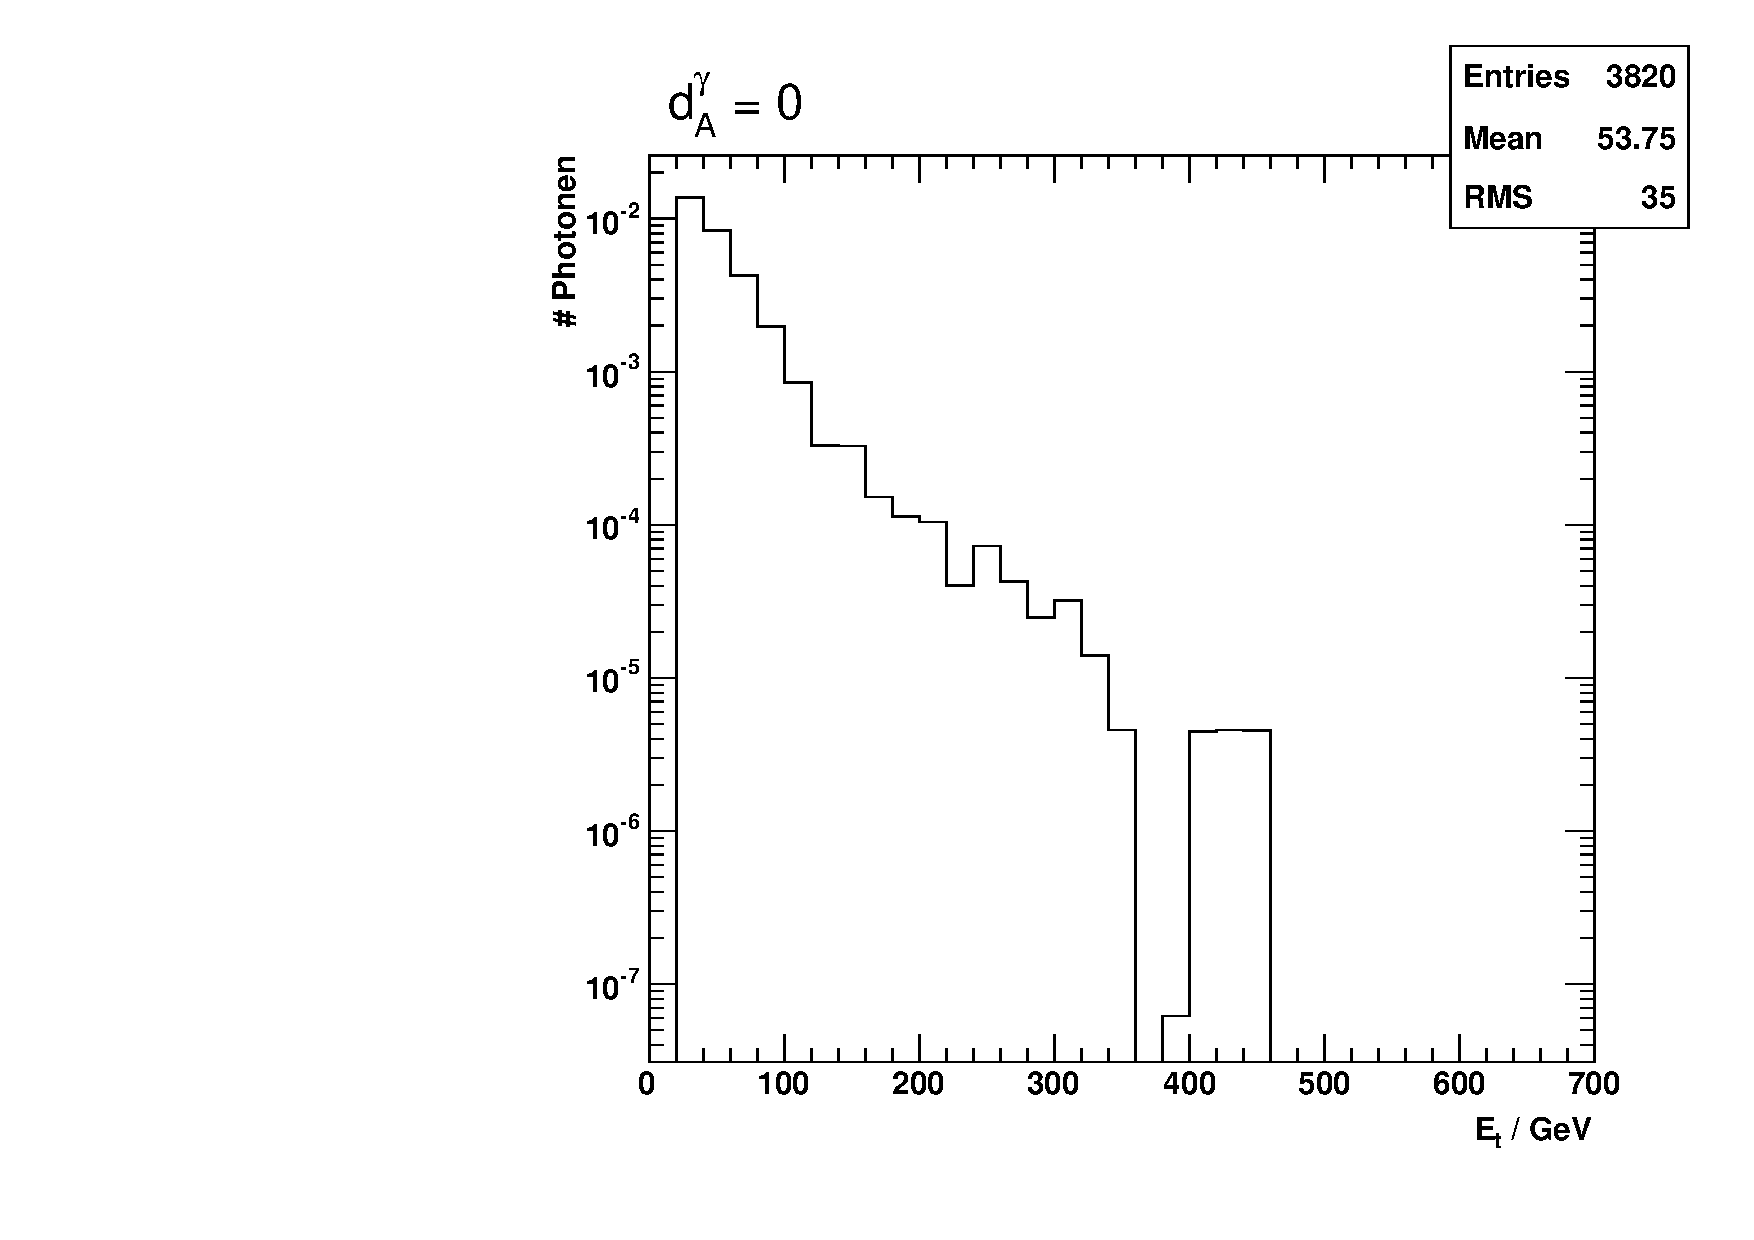
\includegraphics[width=\textwidth]{bilder/et_0.pdf}%
\end{subfigure}
\hspace{0.1\textwidth}
\begin{subfigure}[b]{0.4\textwidth}
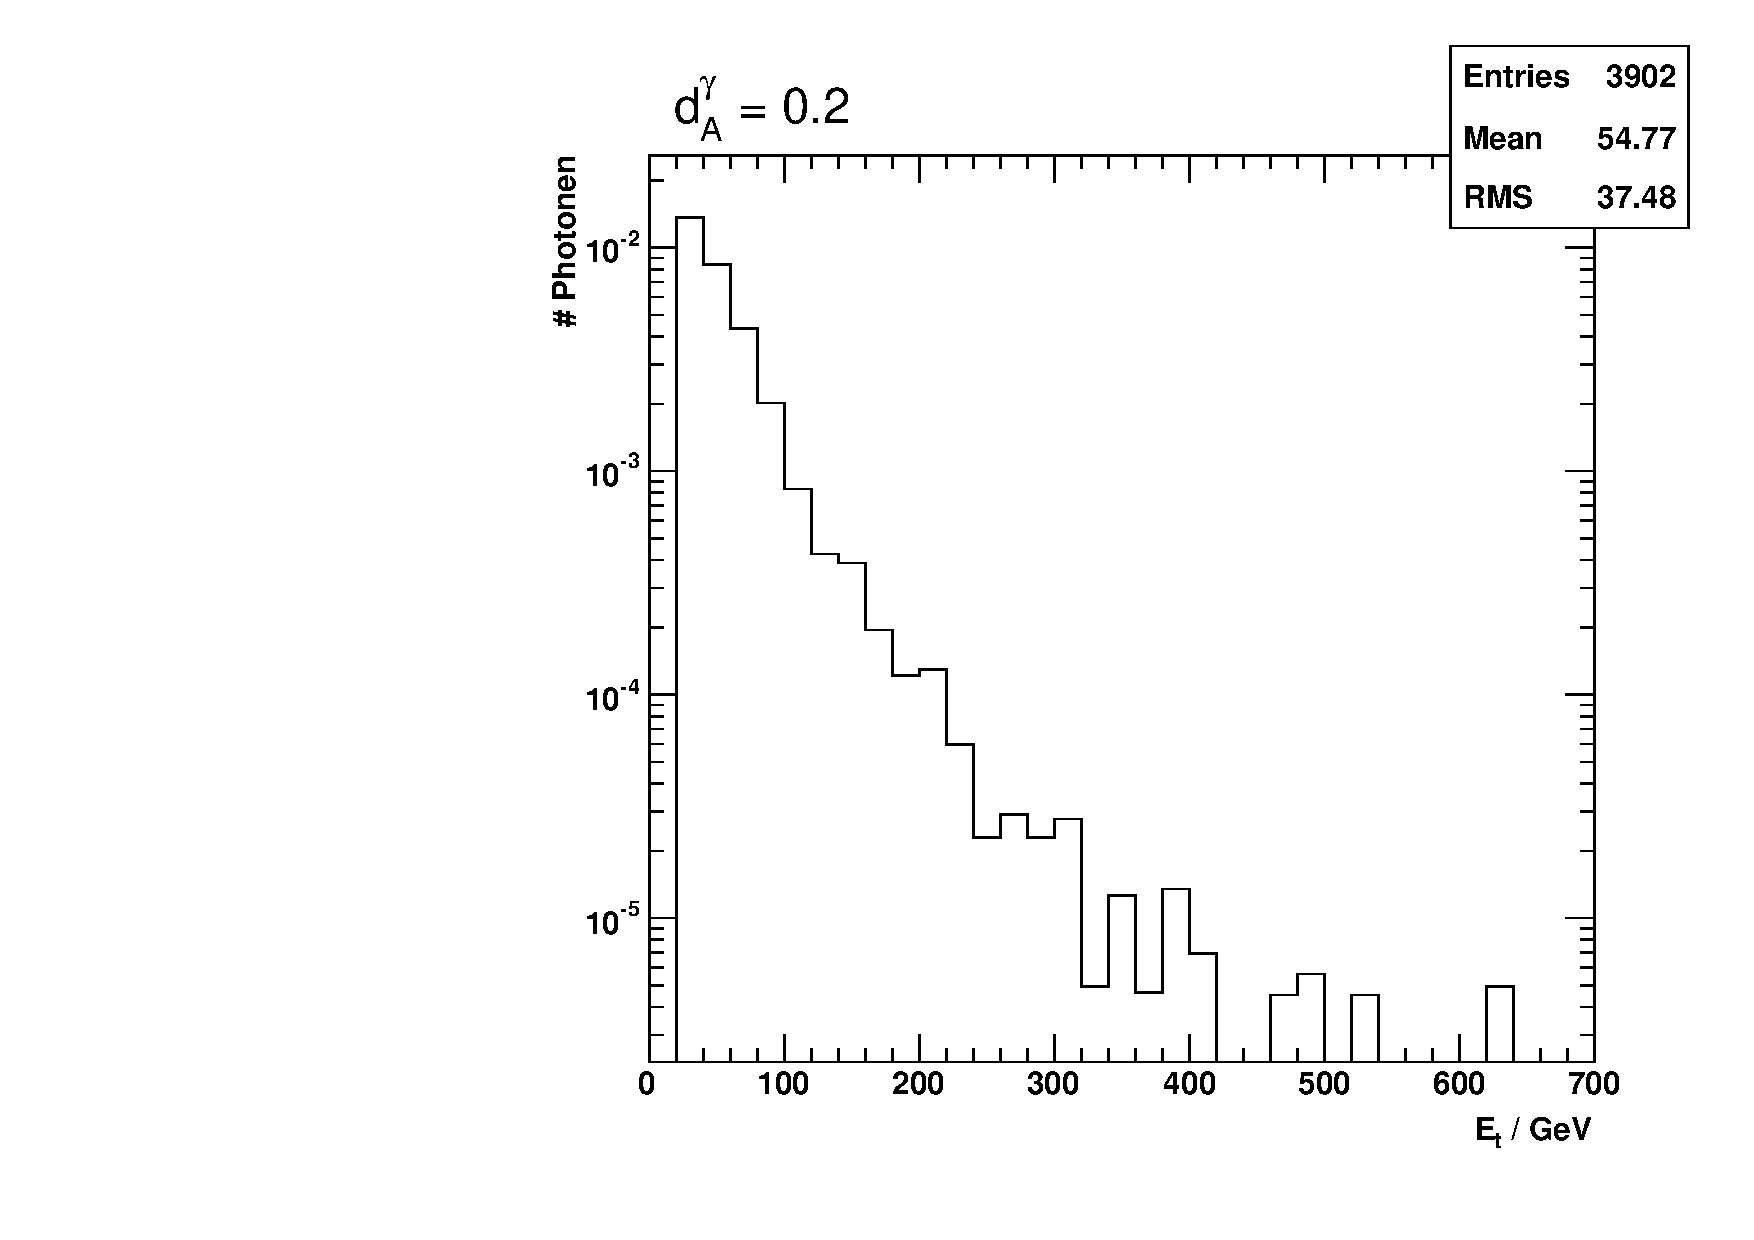
\includegraphics[width=\textwidth]{bilder/et_02.pdf}%
\end{subfigure}

\begin{subfigure}[b]{0.4\textwidth}
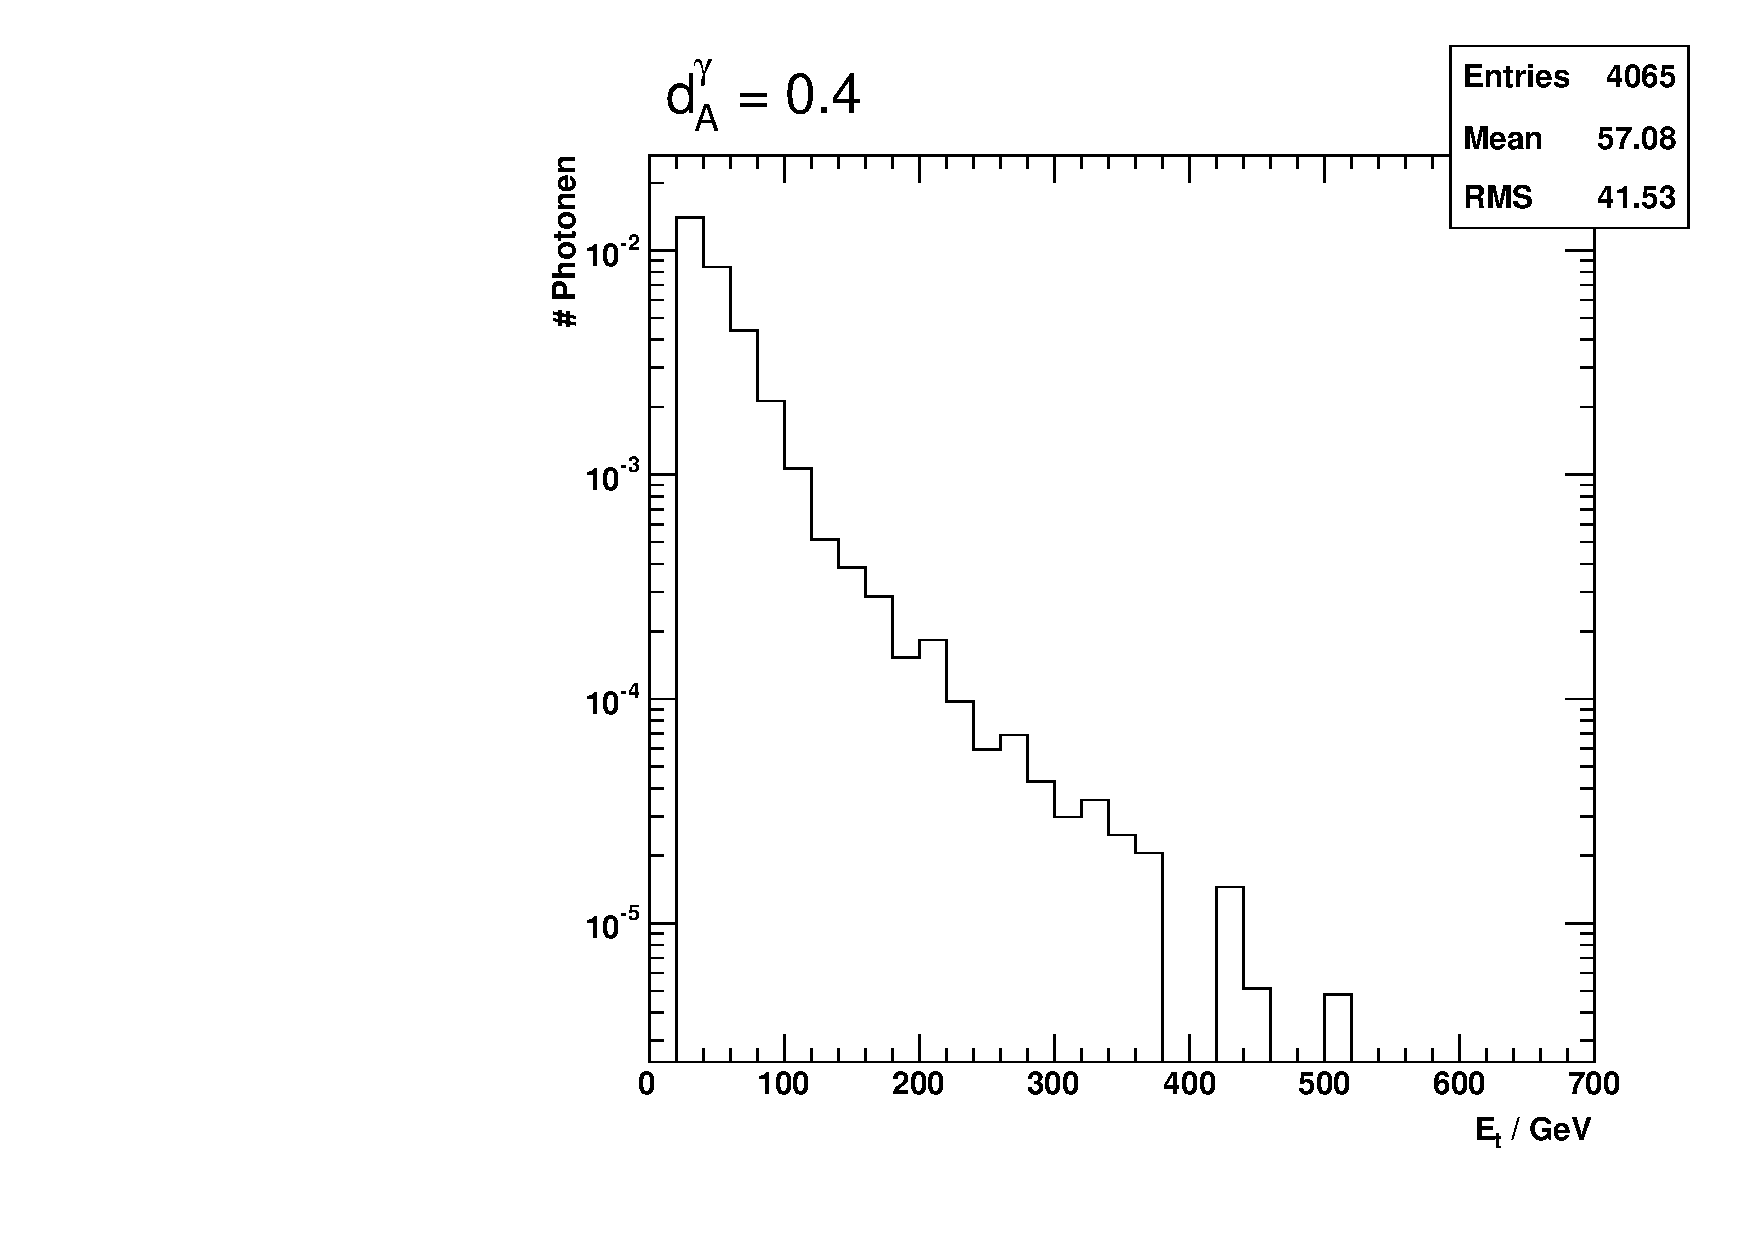
\includegraphics[width=\textwidth]{bilder/et_04.pdf}%
\end{subfigure}
\hspace{0.1\textwidth}
\begin{subfigure}[b]{0.4\textwidth}
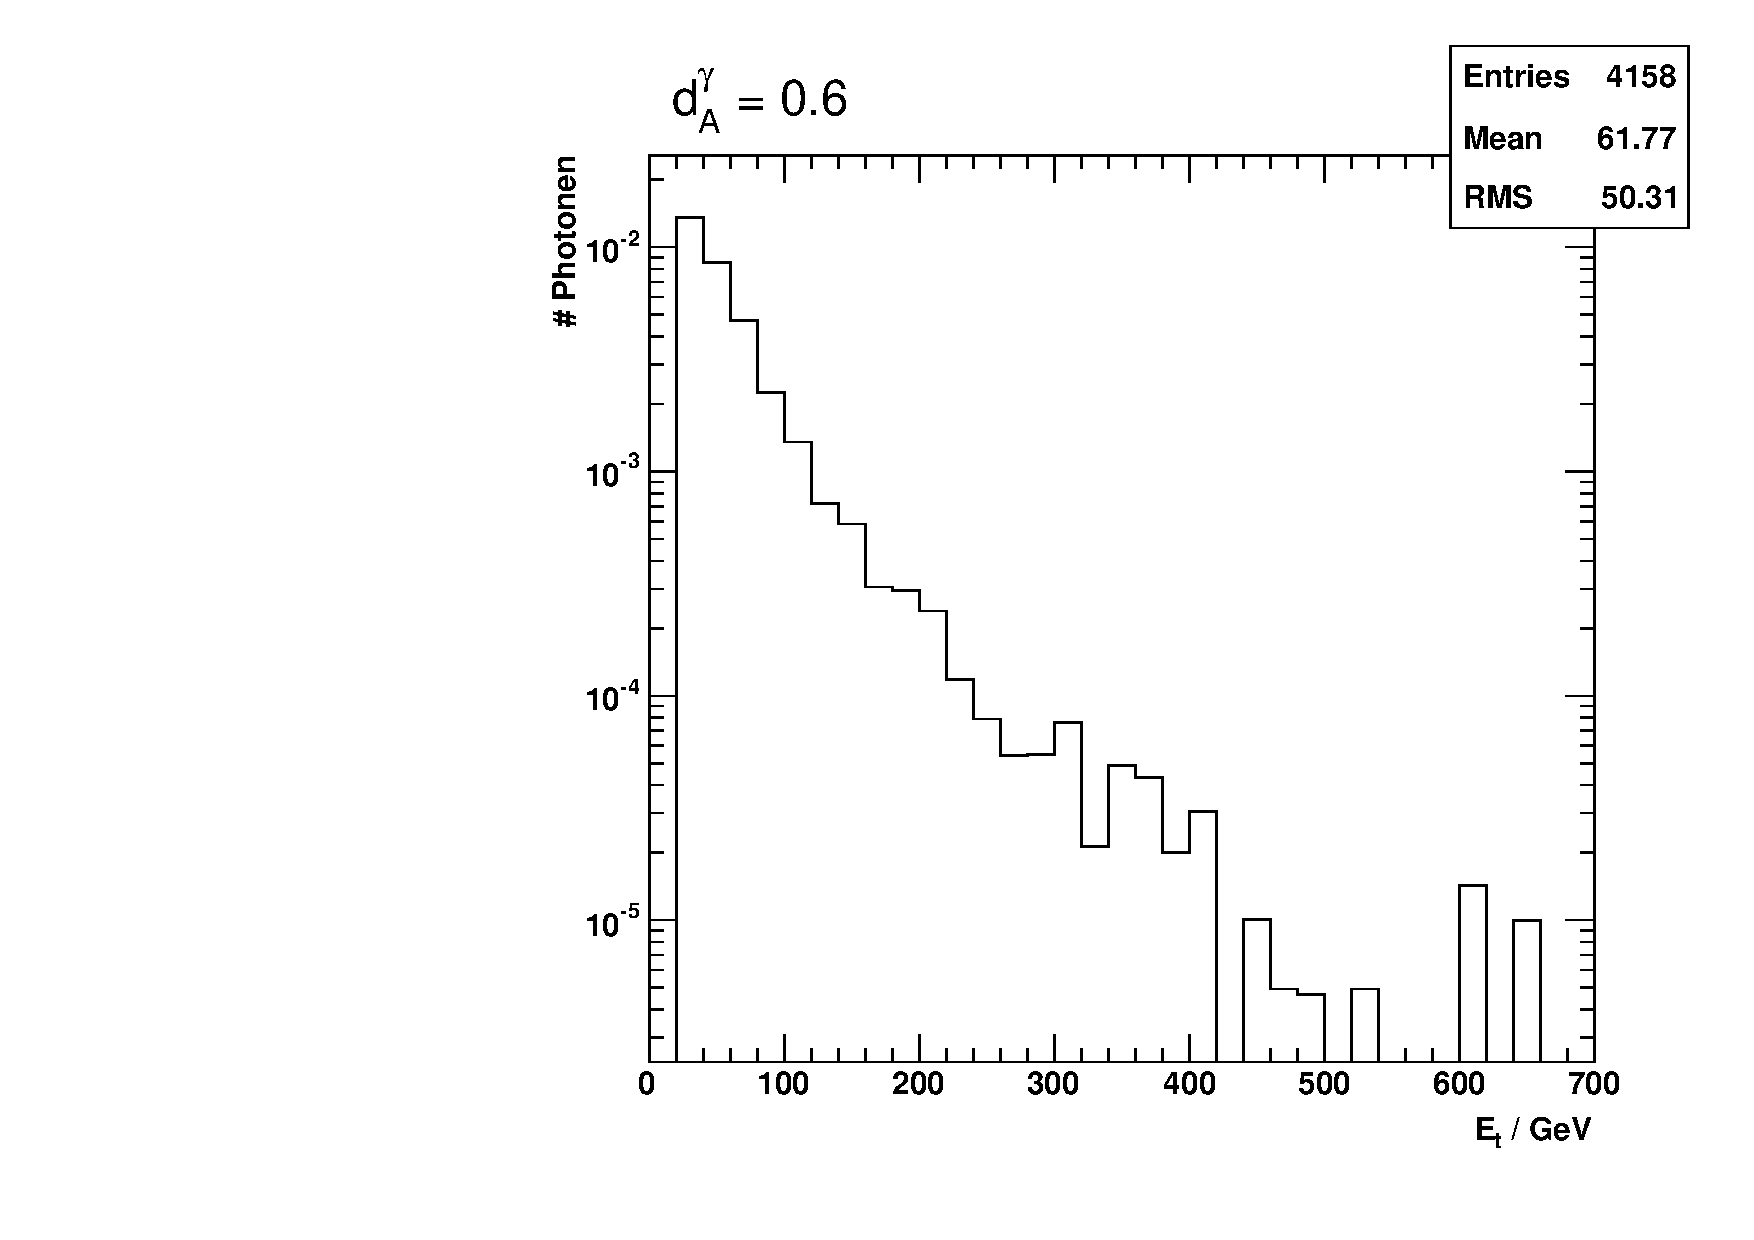
\includegraphics[width=\textwidth]{bilder/et_06.pdf}%
\end{subfigure}

\begin{subfigure}[b]{0.4\textwidth}
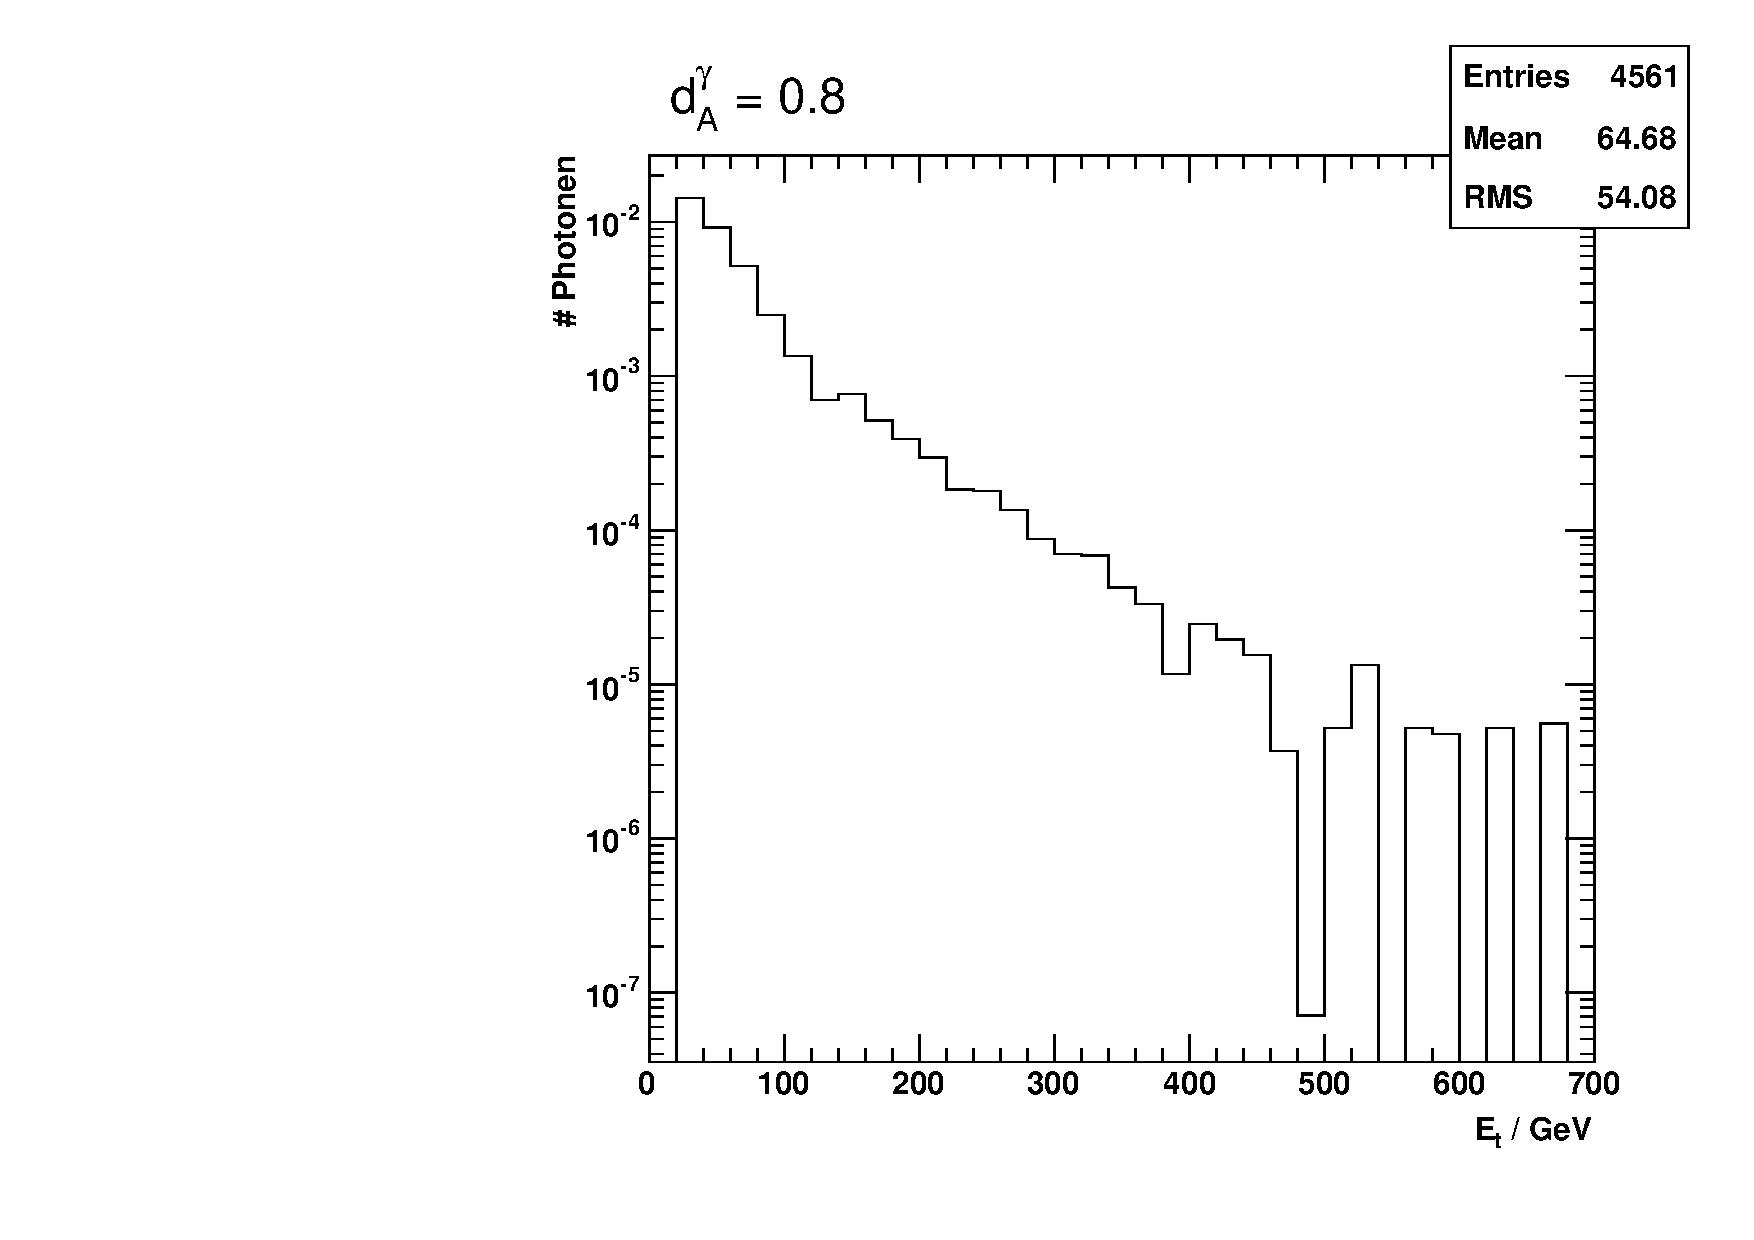
\includegraphics[width=\textwidth]{bilder/et_08.pdf}%
\end{subfigure}
\hspace{0.1\textwidth}
\begin{subfigure}[b]{0.4\textwidth}
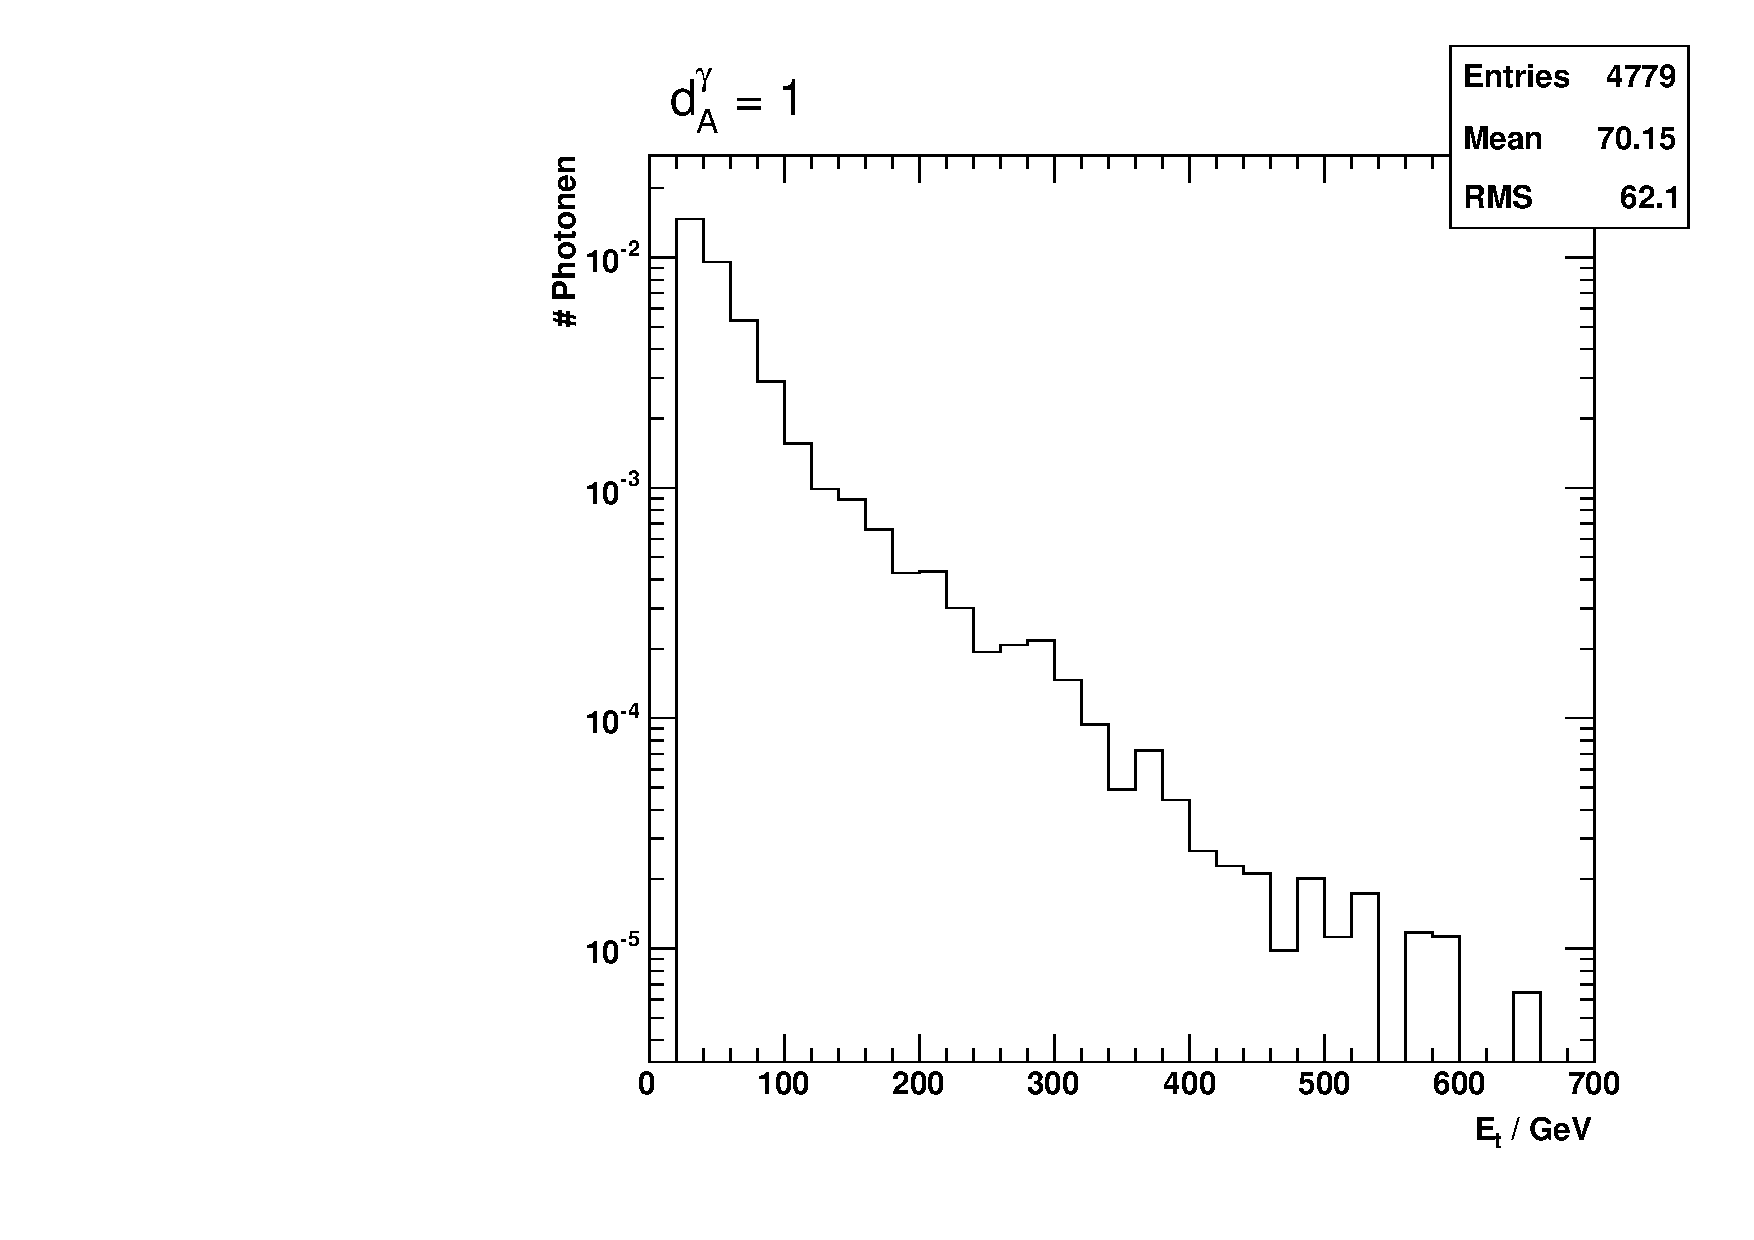
\includegraphics[width=\textwidth]{bilder/et_1.pdf}%
\end{subfigure}
\caption{$E_T$-Verteilungen von rekonstruierten und selektierten Monte-Carlo-Daten f�r verschiedene Werte von $d_A^{\gamma}$.}%
\label{fig:et_galerie}%
\end{figure}

\begin{figure}%
\centering
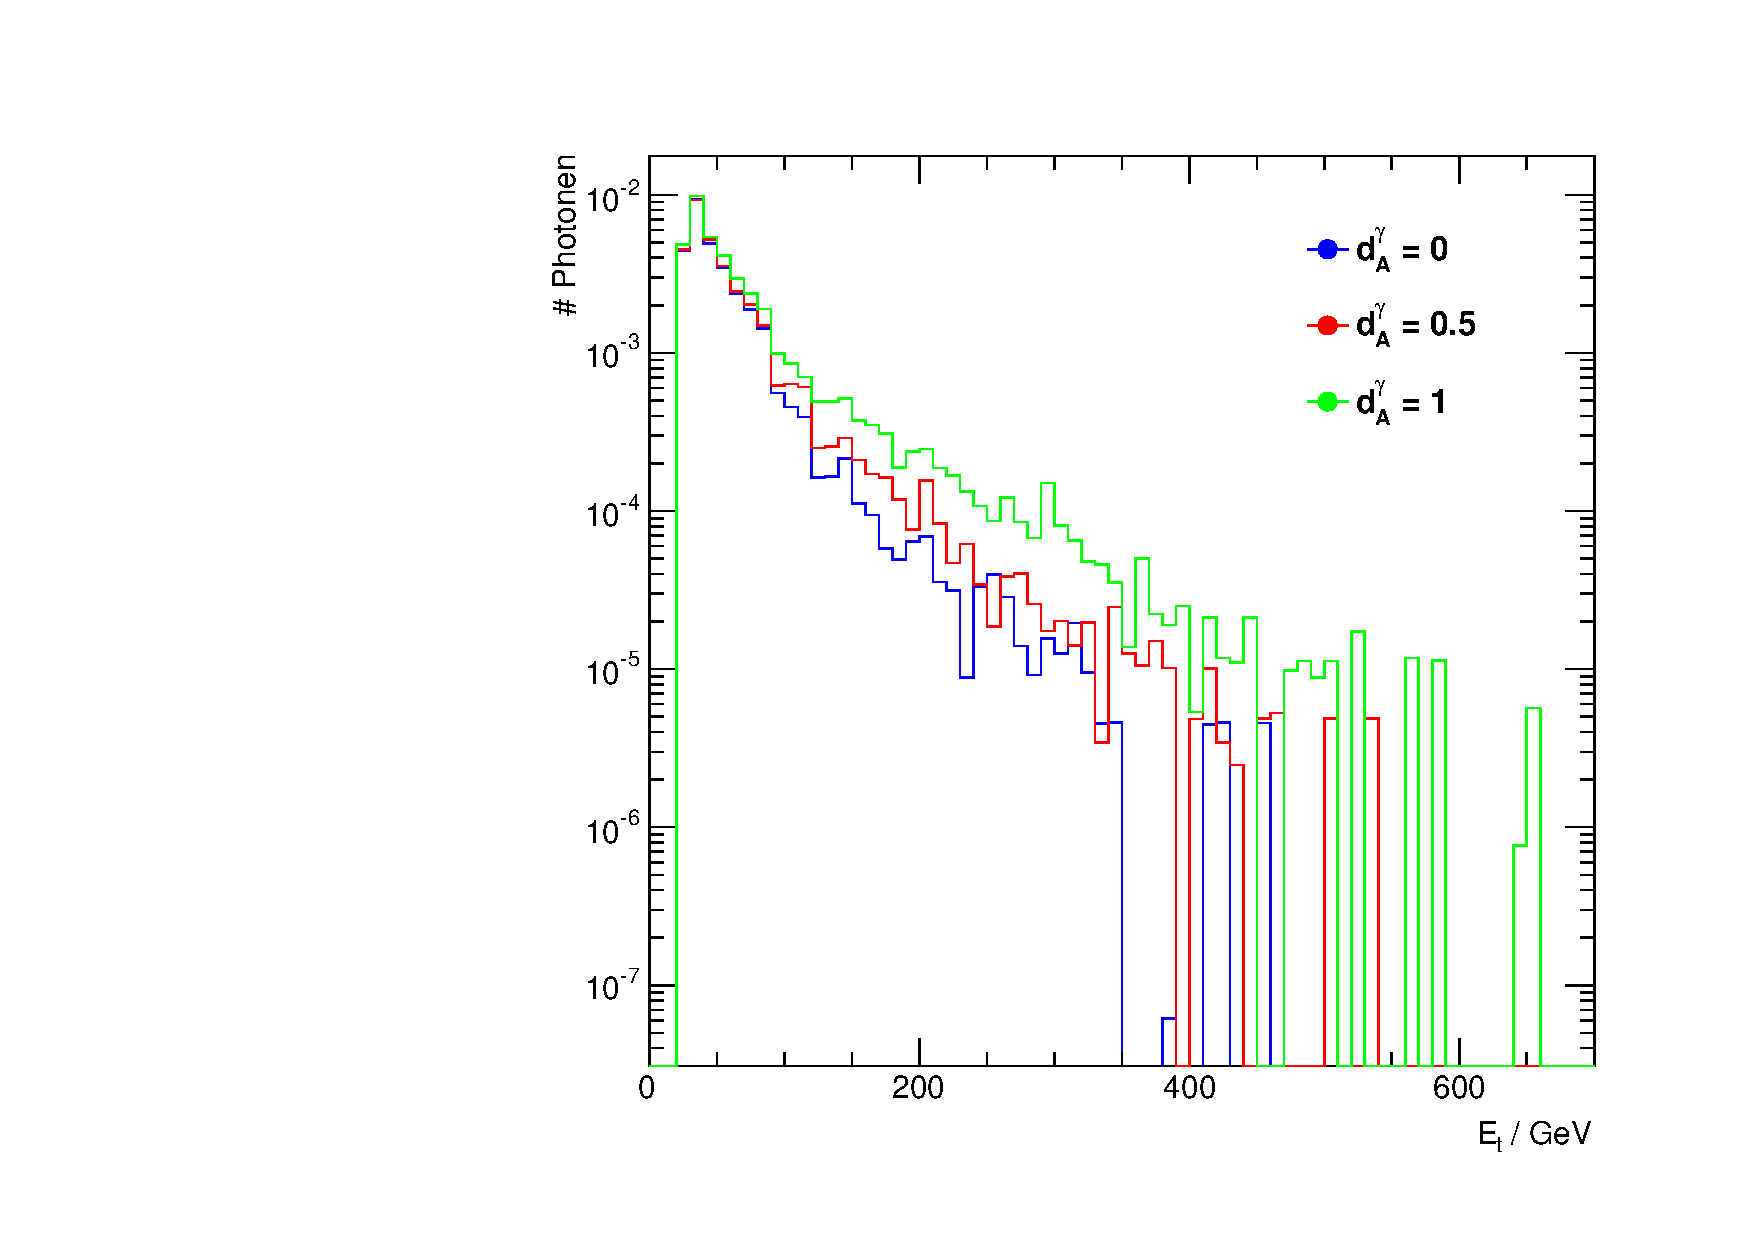
\includegraphics[width=0.6\columnwidth]{bilder/et_kombi}%
\caption{$E_T$-Spektren bei $d_A^{\gamma}=$0; 0,5 und 1.}%
\label{fig:et_kombi}%
\end{figure}

\section{2-Bin-Analyse}

Das $E_T$-Spektrum wird in zwei Bereiche unterteilt, einen niederenergetischen Bereich von 0\,GeV bis 100\,GeV und einen hochenergetischen Bereich von 100\,GeV bis 700\,GeV. Das Verh�ltnis der Ereignisse in den beiden Bereichen wird gegen $d_A^{\gamma}$ aufgetragen, siehe Abbildung \ref{fig:twobin_reco_plot}. Die $E_{Low}/E_{High}$-Werte und die Unsicherheiten sind hier zwischen den Messwerten interpoliert. Man erkennt auch auf Rekonstruktionsniveau eine klare Abh�ngigkeit des Verh�ltnisses $E_{Low}/E_{High}$ von der Kopplungsst�rke $d_A^{\gamma}$. Ebenso ist auch hier wie auf Generatorniveau eine gute Separationskraft erkennbar, die Werte reichen von $E_{Low}/E_{High} = 6,4$ bei $d_A^{\gamma} = 0$ bis $E_{Low}/E_{High} = 3,2$ bei $d_A^{\gamma} = 1$. Die Unsicherheit auf den Messwert liegt im Bereich von $\Delta E_{Low}/E_{High} < 0,3$.

\begin{figure}%
\centering
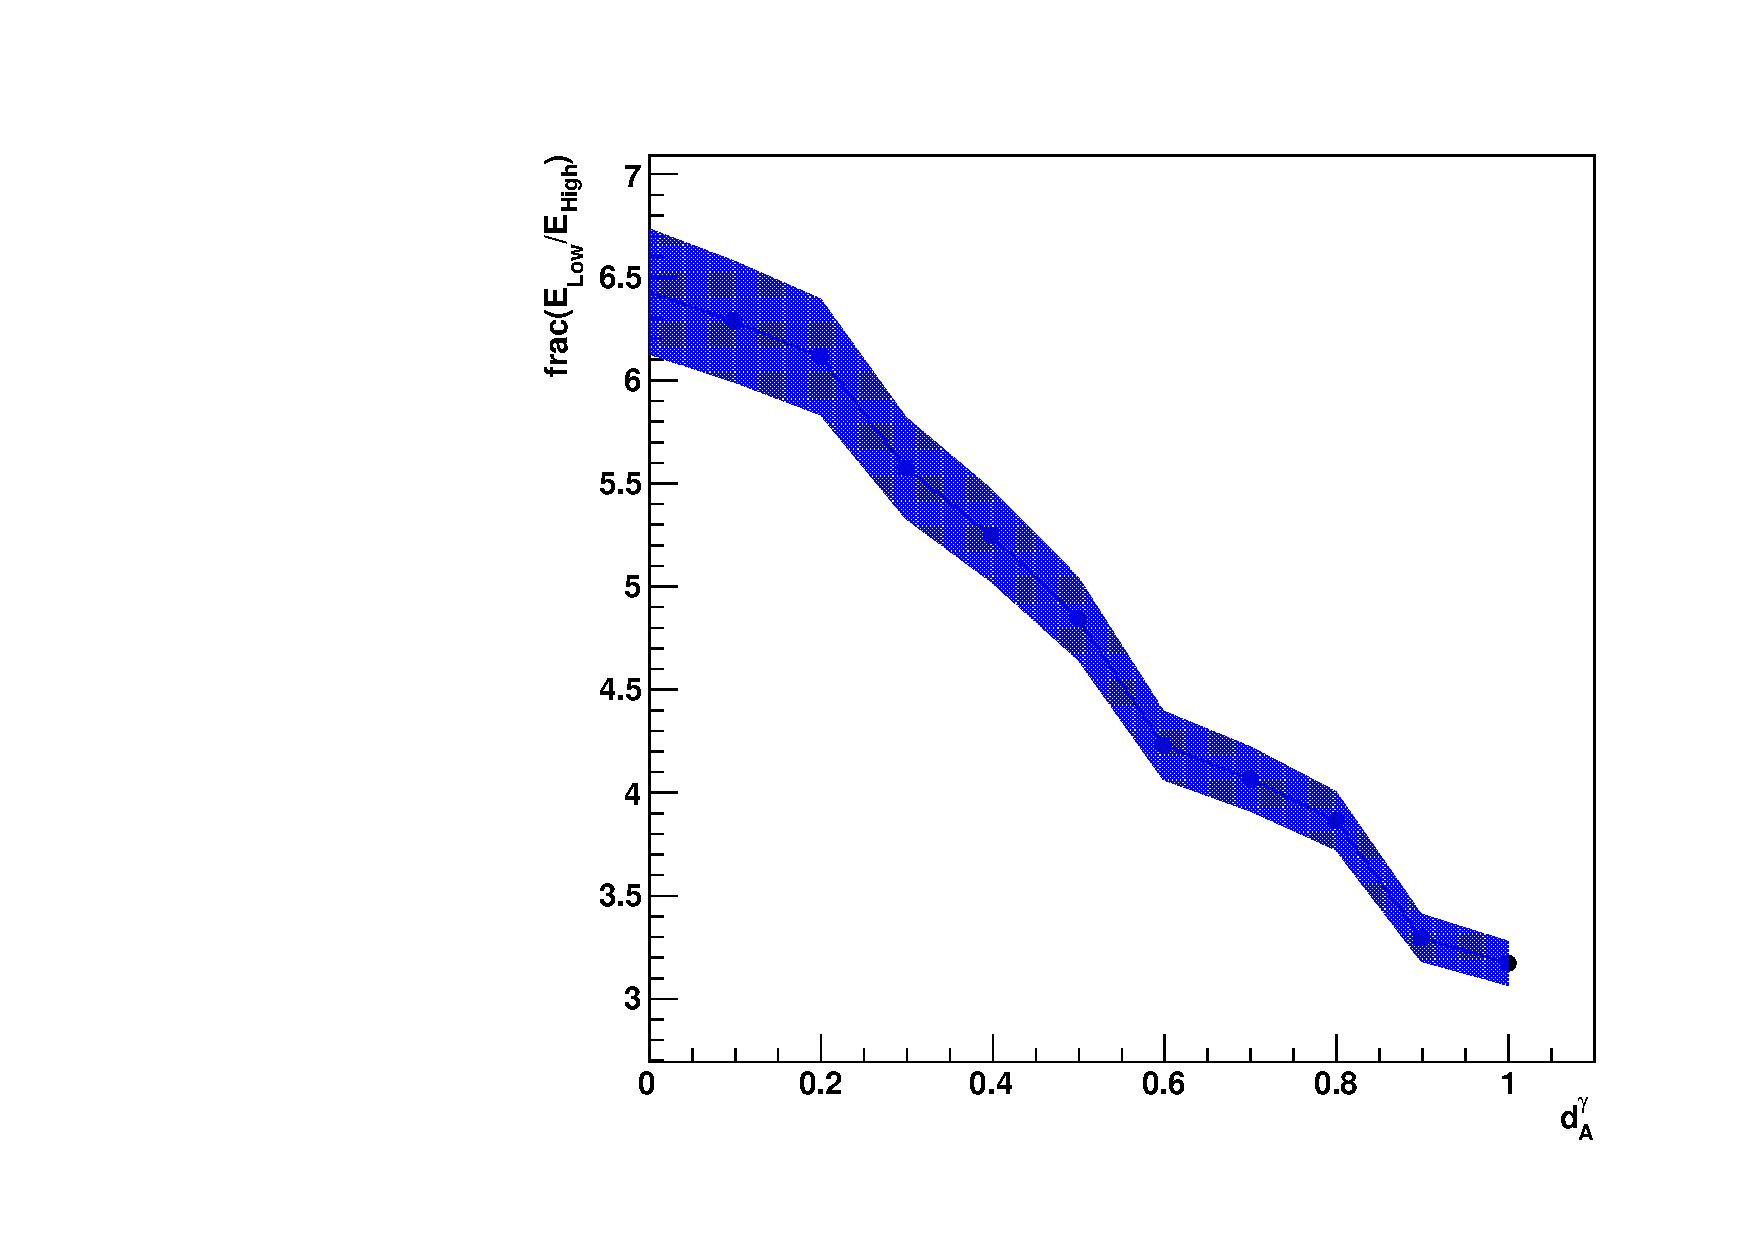
\includegraphics[width=0.5\columnwidth]{bilder/twobin_reco_plot.pdf}%
\caption{}%
\label{fig:twobin_reco_plot}%
\end{figure}

\section{\texorpdfstring{$E_T$}{ET}-Mean-Analyse}

Die Schwerpunkte der $E_T$-Spektren der Photonkandidaten sowie die Unsicherheiten werden mittels der Gleichungen \ref{eq:mean} sowie \ref{eq:meanerror} bestimmt und gegen $d_A^{\gamma}$ aufgetragen. Auch hier bleibt die Abh�ngigkeit des Schwerpunktes von $d_A^{\gamma}$ auf Rekonstruktionslevel erhalten (siehe Abbildung \ref{fig:mean_reco_plot}. Die Werte liegen dabei zwischen $\overline{E_T} = 53,75$\,GeV und $\overline{E_T} = 70,15$\,GeV bei einer Unsicherheit von $\Delta \overline{E_T} < 1,9$\,GeV.

\begin{figure}%
\centering
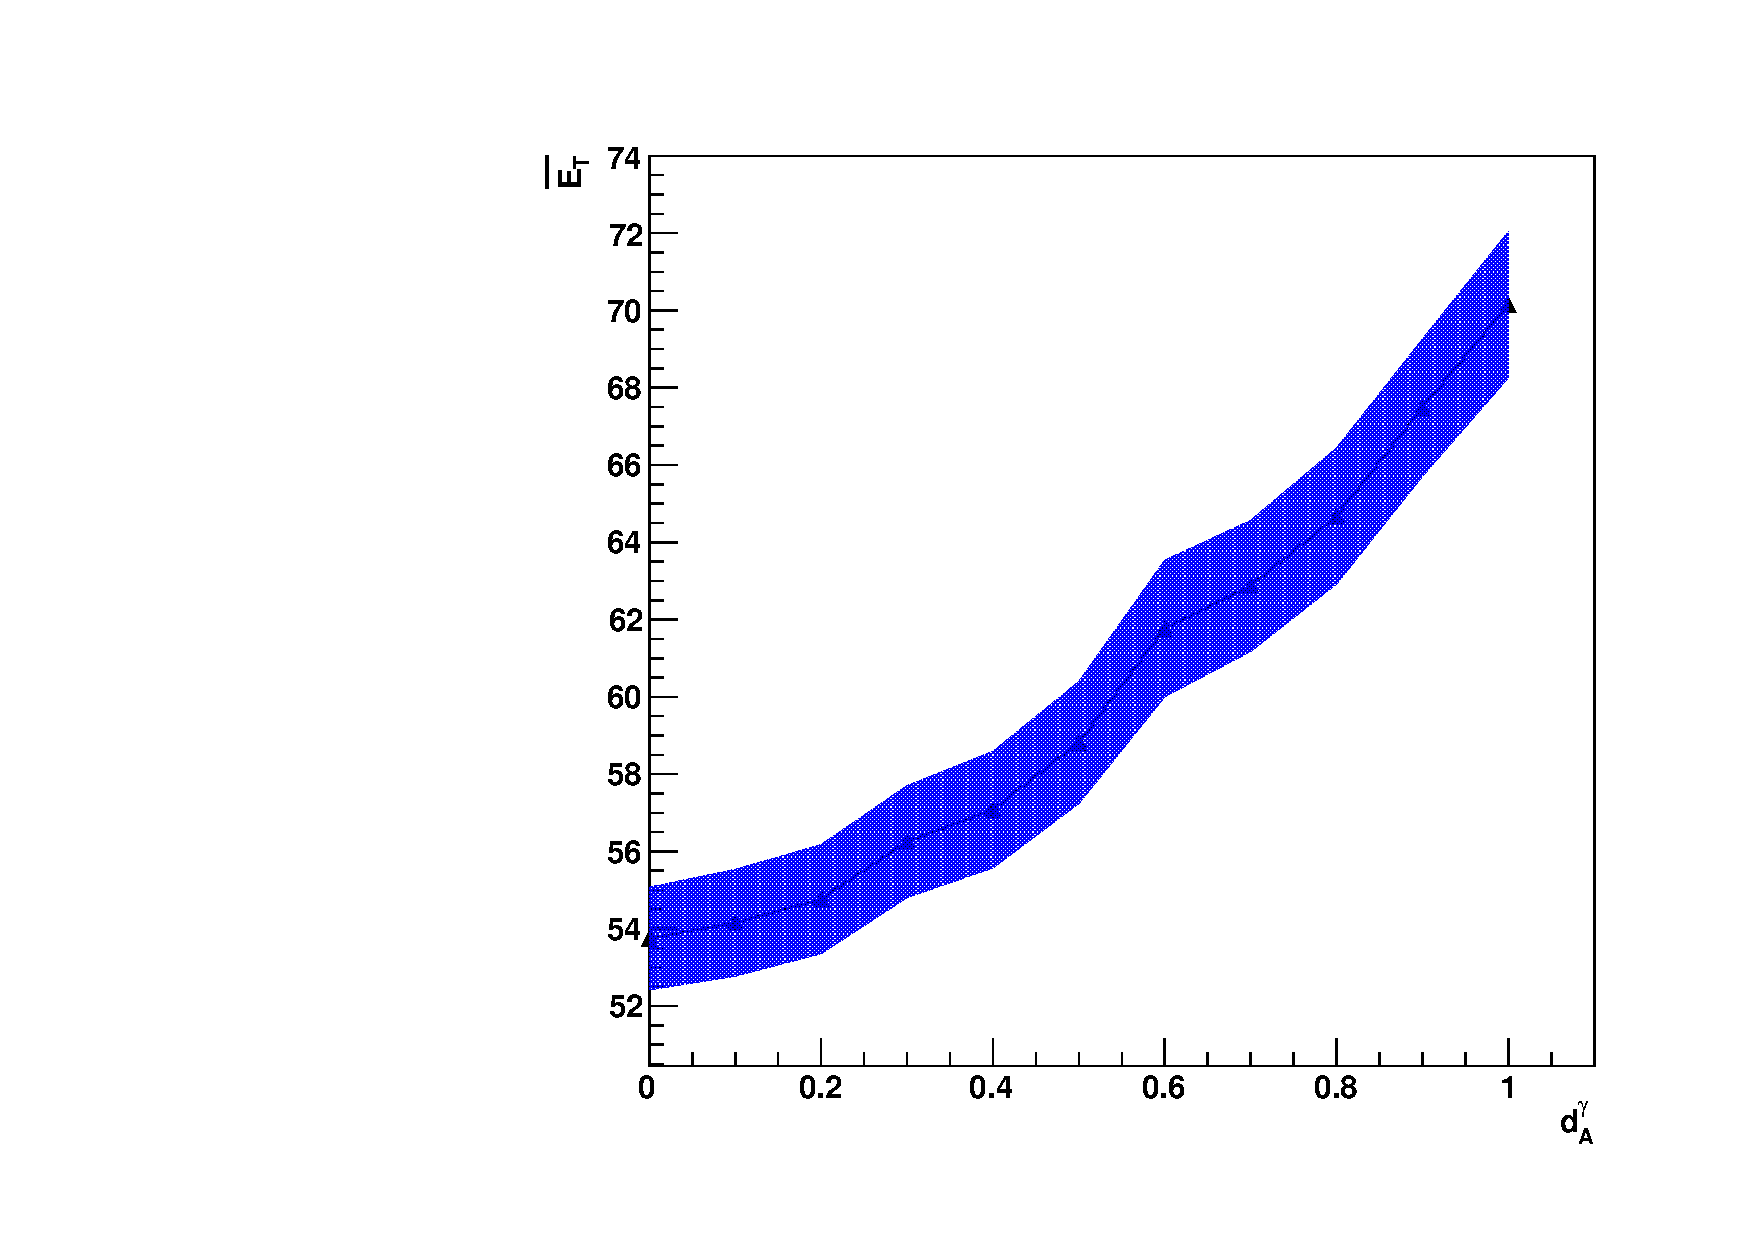
\includegraphics[width=0.5\columnwidth]{bilder/mean_reco_plot.pdf}%
\caption{}%
\label{fig:mean_reco_plot}%
\end{figure}

\section{Analyse der Exponentialanpassung der \texorpdfstring{$E_T$}{ET}-Verteilung}

Die Anpassung einer Exponentialfunktion an die $E_T$-Verteilung des Photons wird betrachtet. Dazu wird das $E_T$-Spektrum im Bereich von 20\,GeV bis 200\,GeV durch eine Exponentialfunktion wie in Gleichung \ref{eq:expofit} beschrieben angepasst, siehe Abbildung \ref{fig:fit_galerie}. Der Wert f�r $\lambda$ wird gegen $d_A^{\gamma}$ aufgetragen, siehe Abbildung \ref{fig:slope_reco_plot}. Wie in den beiden anderen Analysestrategien bleibt die Abh�ngigkeit der Variablen von $d_A^{\gamma}$ auf Rekonstruktionsniveau erhalten, bei $d_A^{\gamma} = 0,7$ ist jedoch ein Knick im ansonsten streng monoton steigenden Verlauf des $\gamma$-Parameters zu erkennen. Dieser liegt jedoch innerhalb der Unsicherheit. Es werden Werte von $\lambda = -0,035$ f�r $d_A^{\gamma} = 0$ bis $\lambda = -0,024$ f�r $d_A^{\gamma} = 1$ bei einer Unsicherheit von $\Delta \lambda < 0,0007$ gemessen.

\begin{figure}%
\begin{subfigure}[b]{0.4\textwidth}
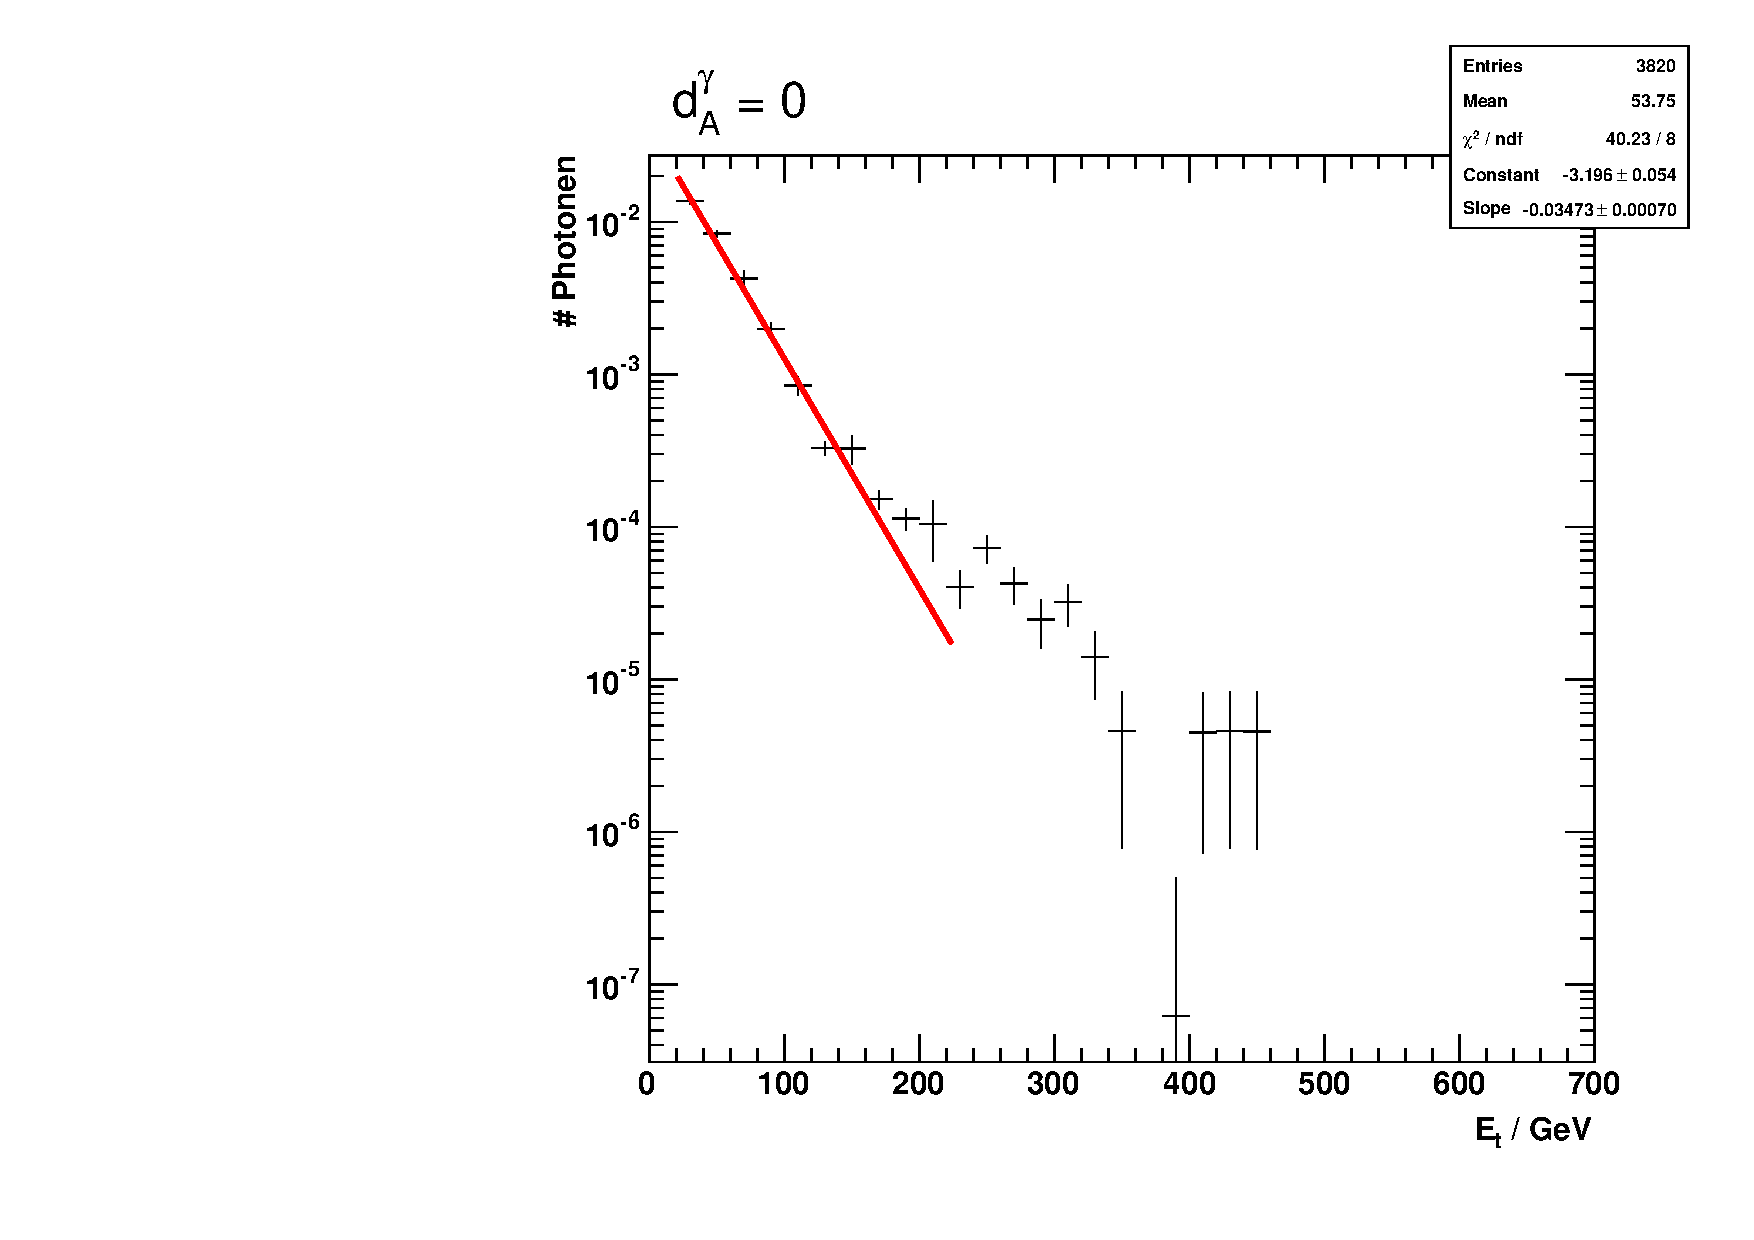
\includegraphics[width=\textwidth]{bilder/fit_0.pdf}%
\end{subfigure}
\hspace{0.1\textwidth}
\begin{subfigure}[b]{0.4\textwidth}
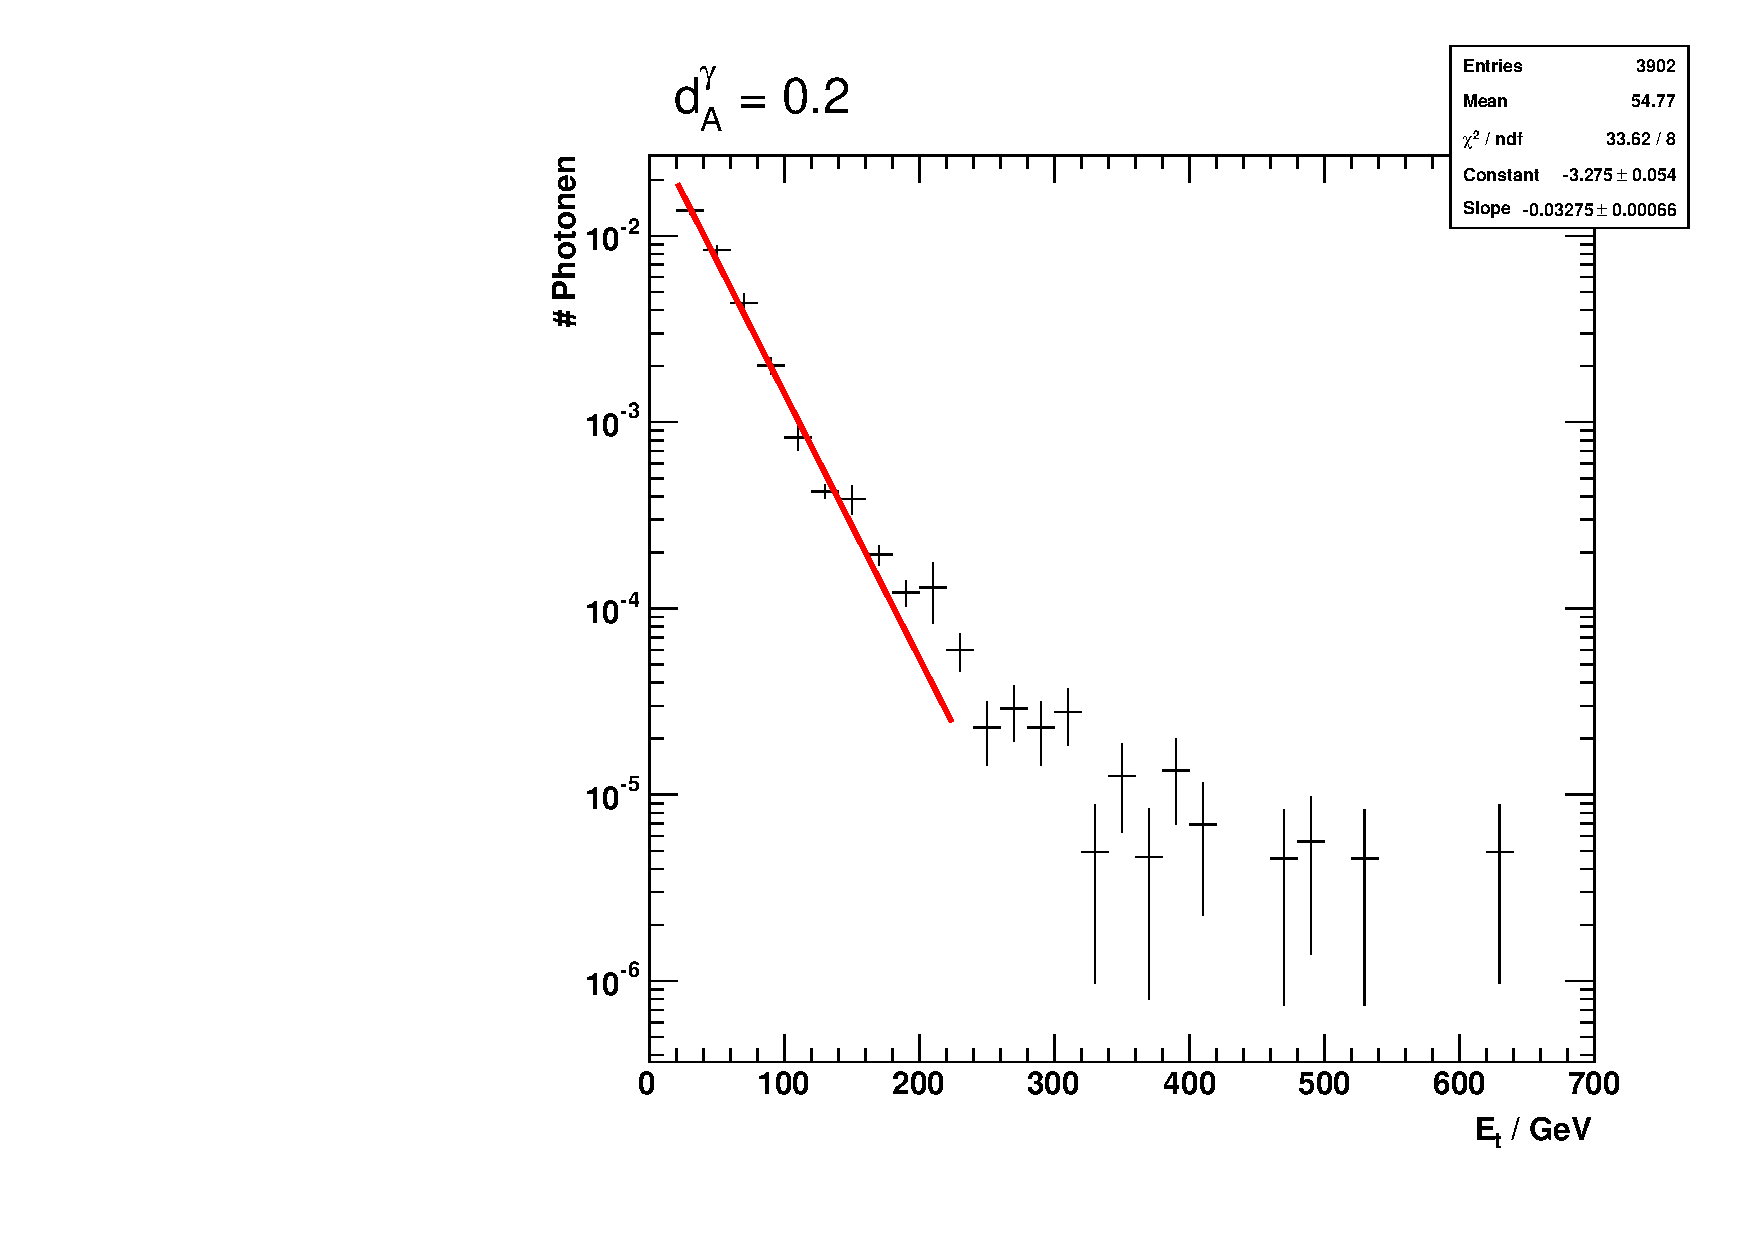
\includegraphics[width=\textwidth]{bilder/fit_02.pdf}%
\end{subfigure}

\begin{subfigure}[b]{0.4\textwidth}
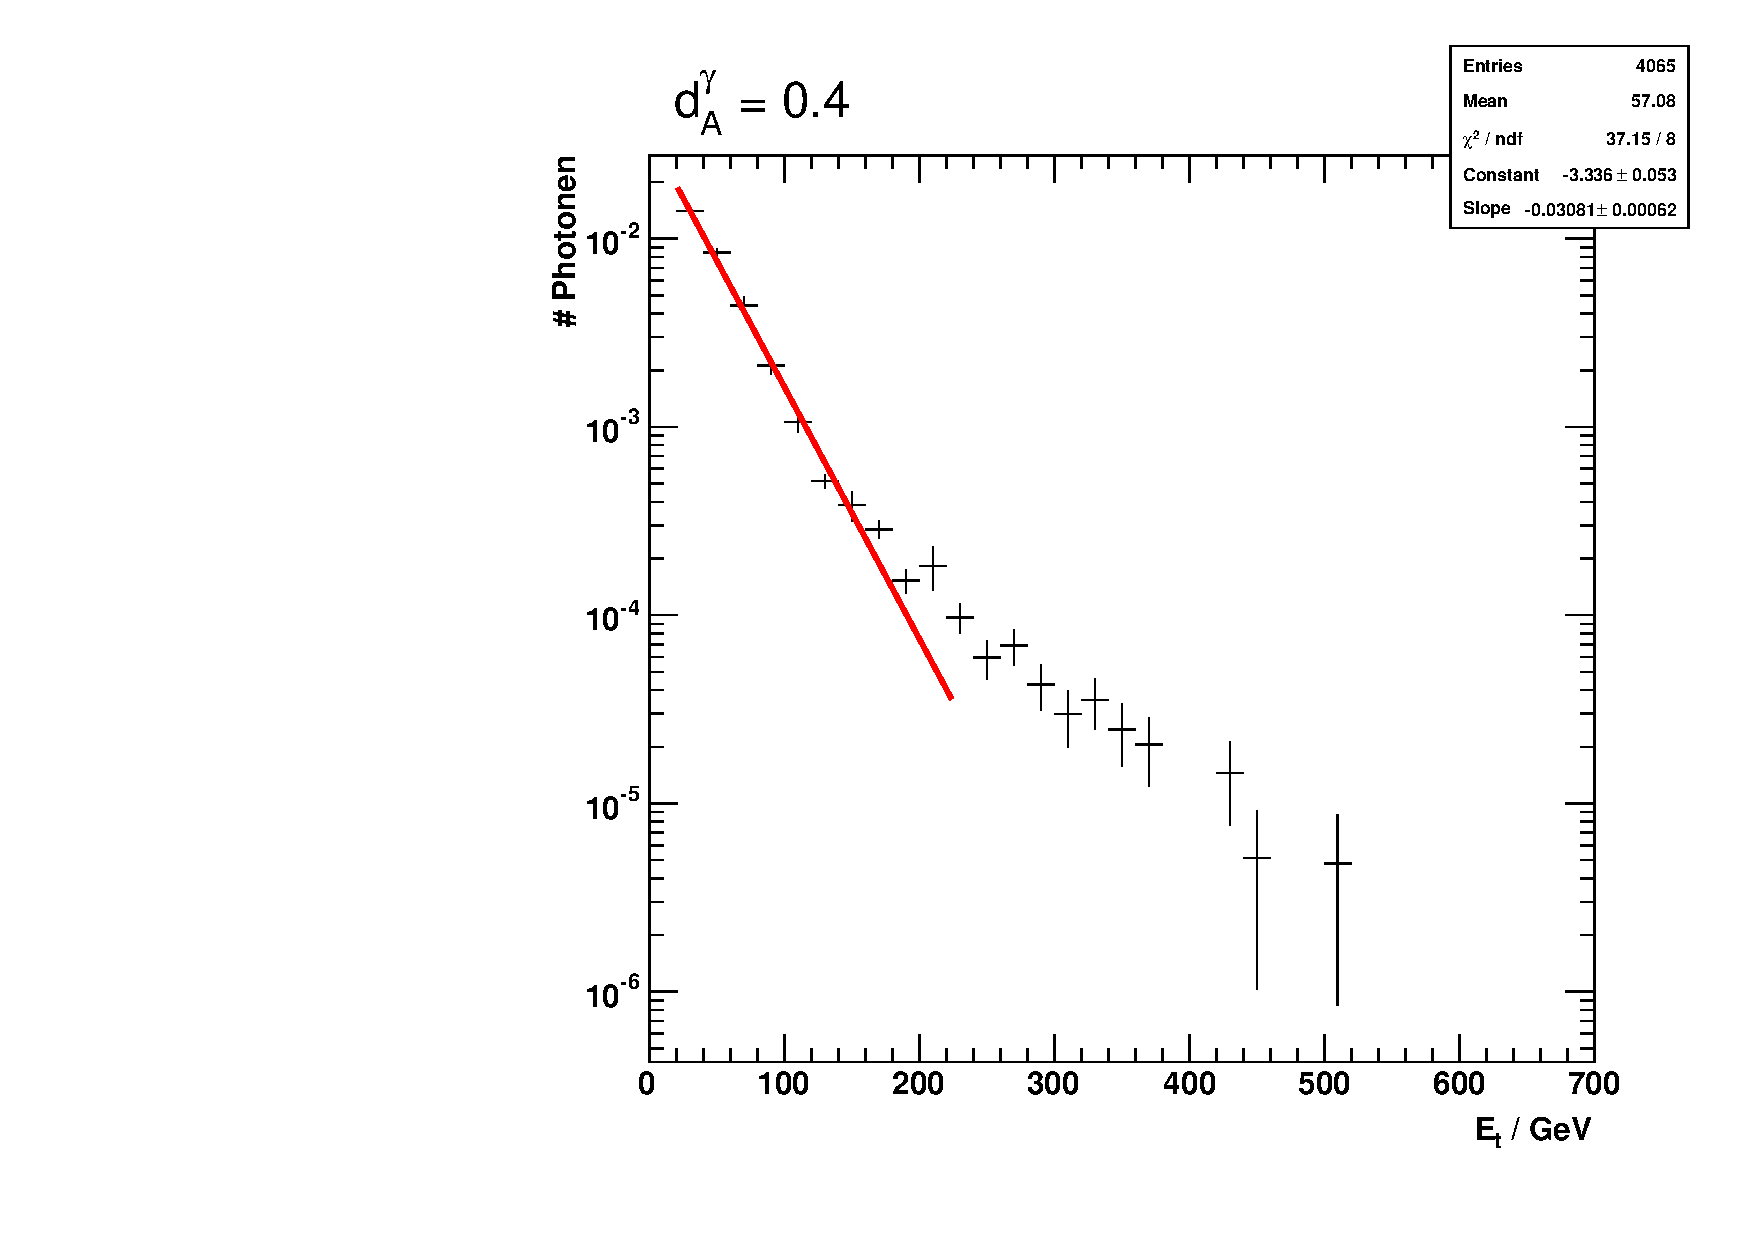
\includegraphics[width=\textwidth]{bilder/fit_04.pdf}%
\end{subfigure}
\hspace{0.1\textwidth}
\begin{subfigure}[b]{0.4\textwidth}
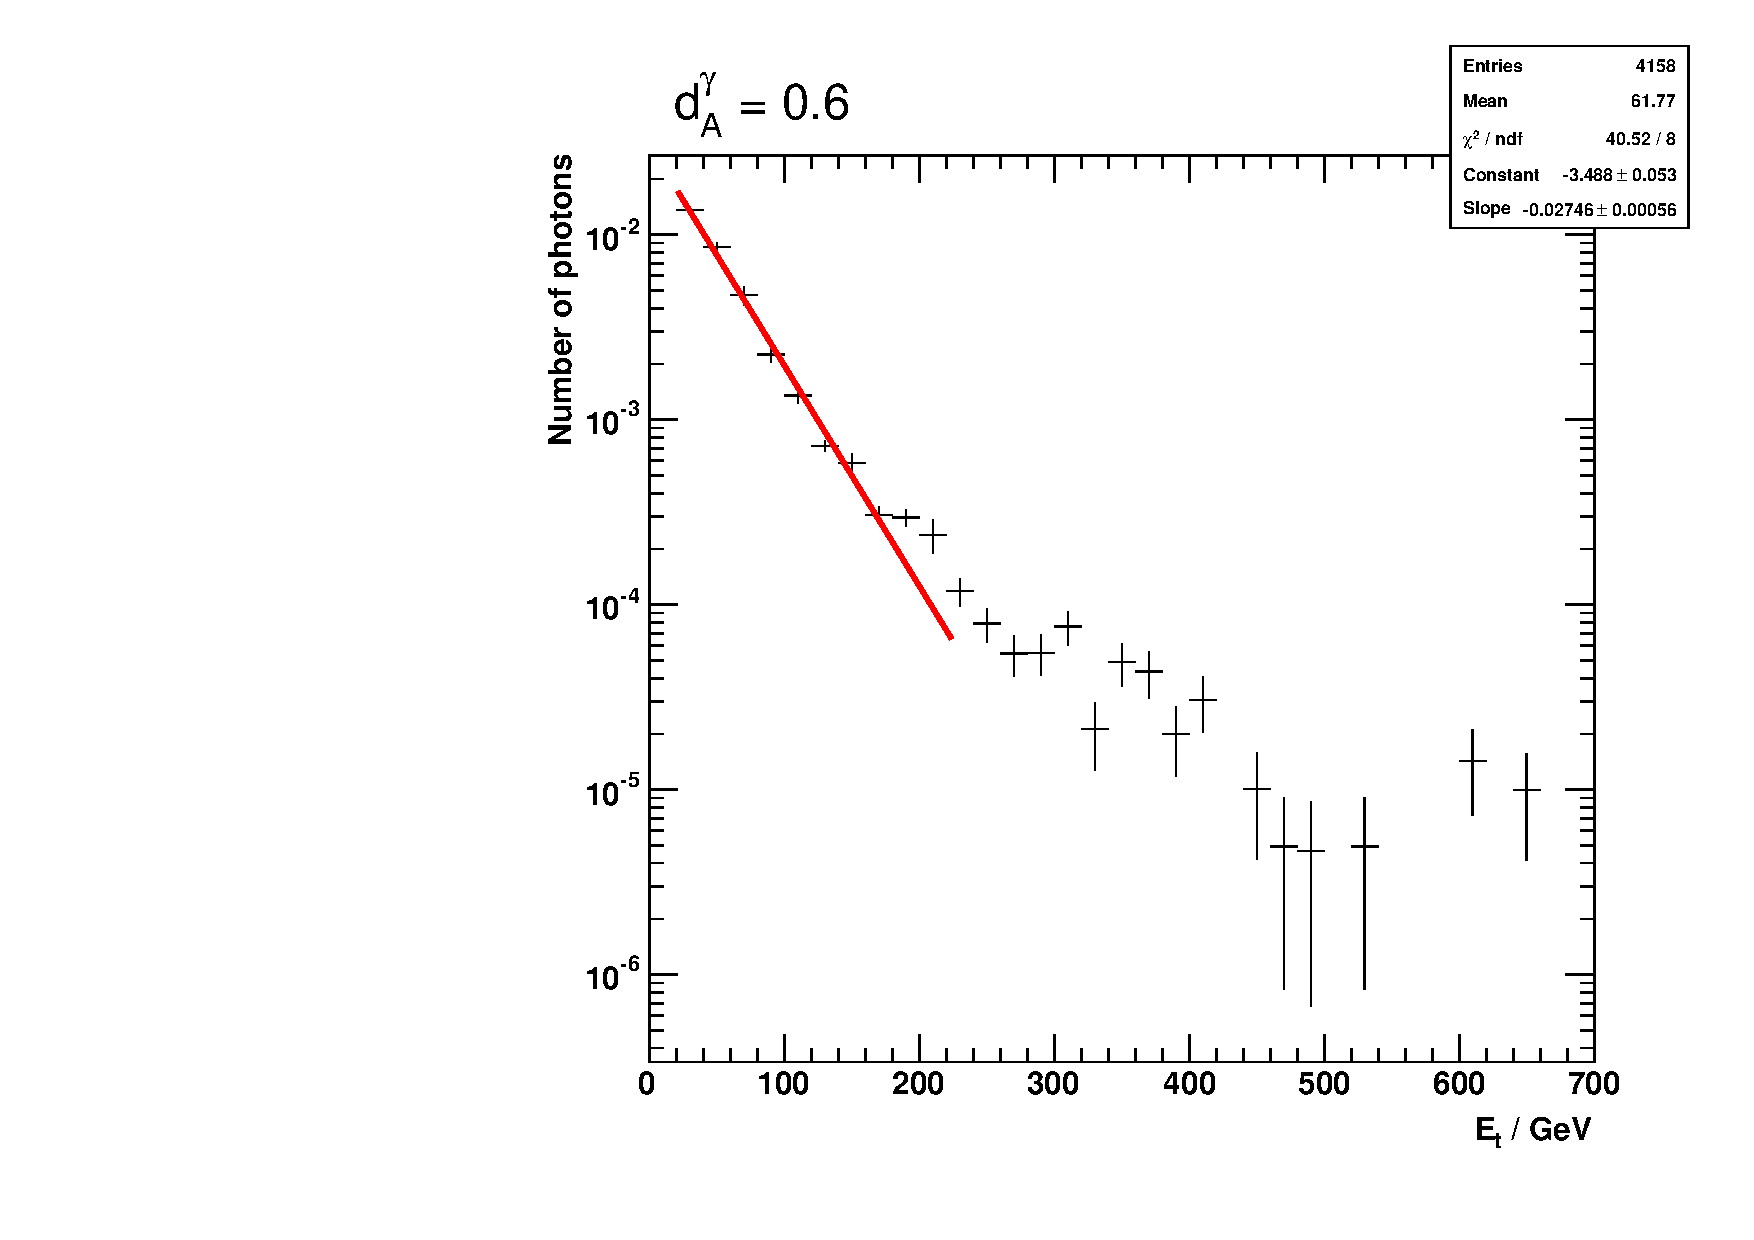
\includegraphics[width=\textwidth]{bilder/fit_06.pdf}%
\end{subfigure}

\begin{subfigure}[b]{0.4\textwidth}
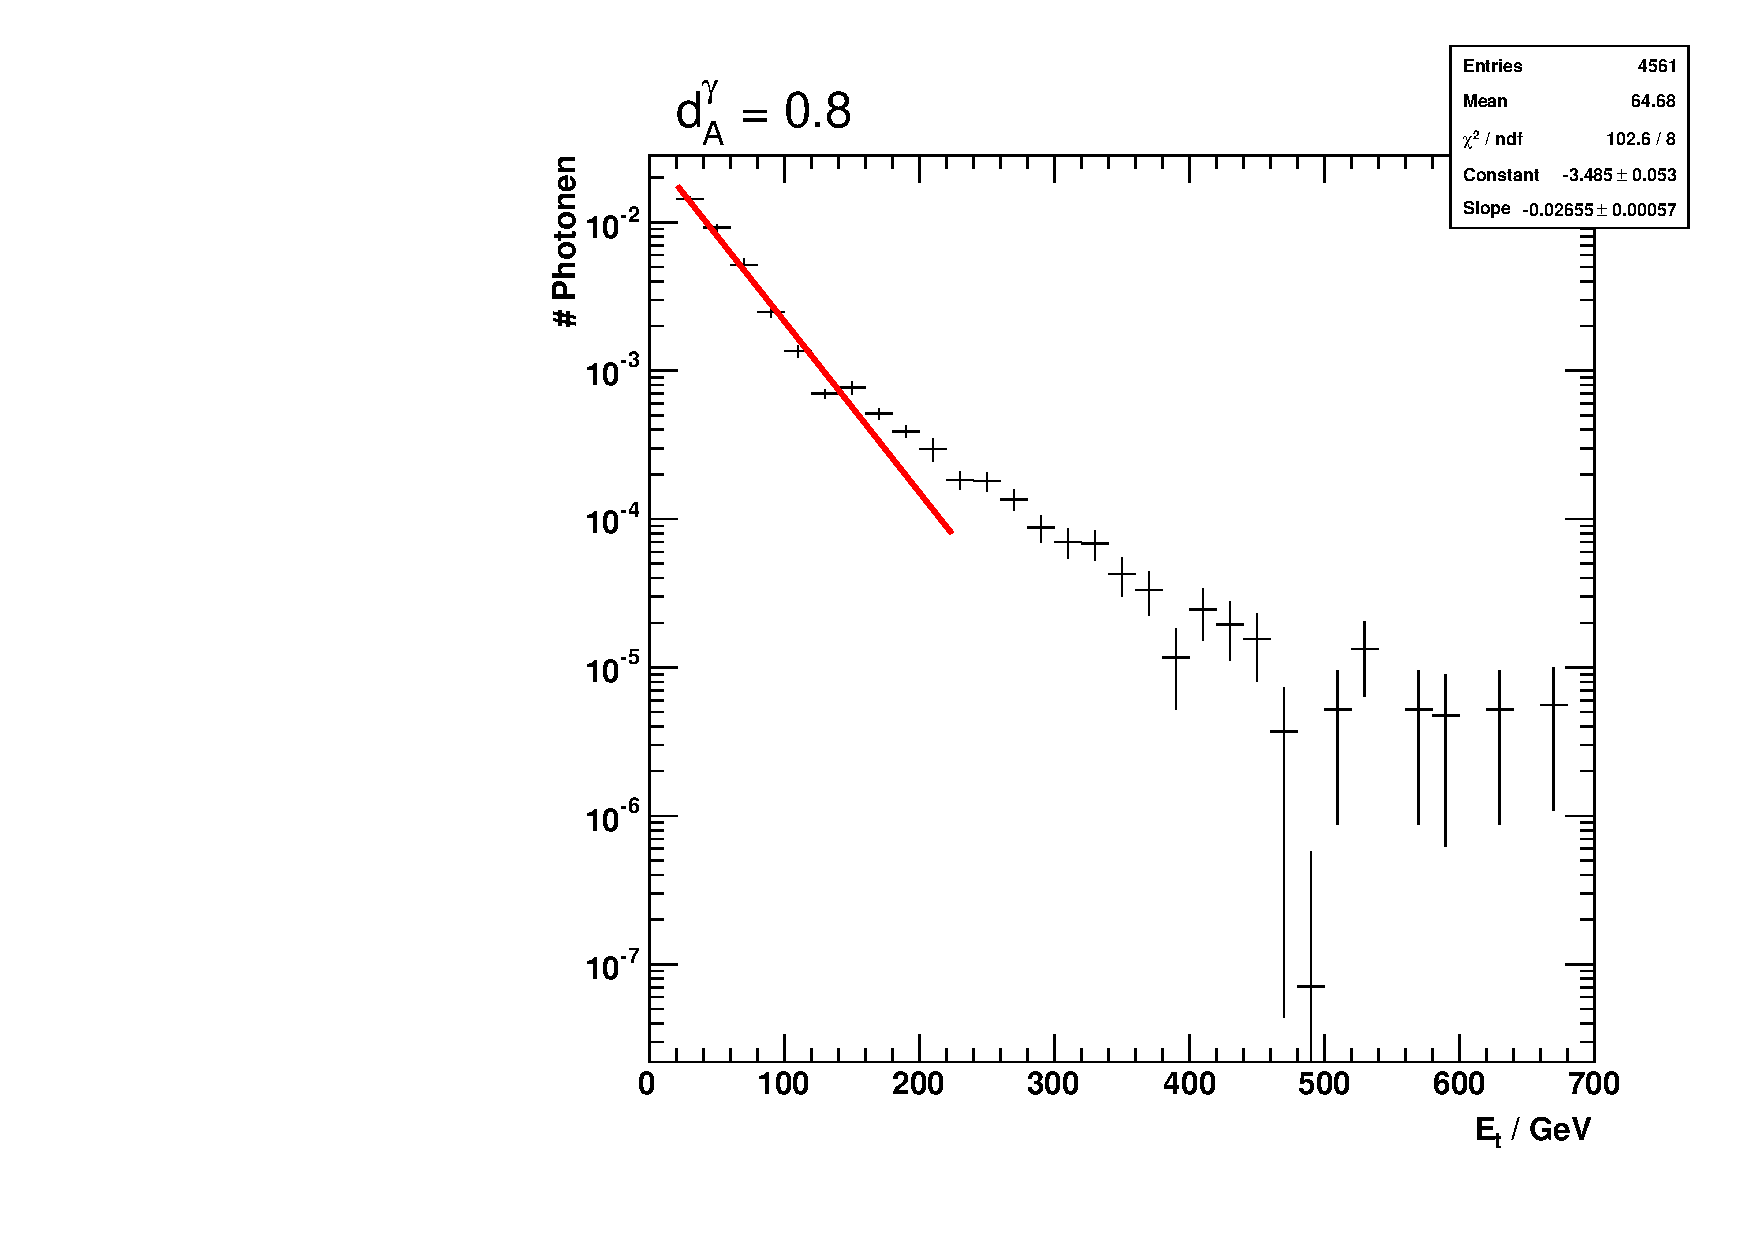
\includegraphics[width=\textwidth]{bilder/fit_08.pdf}%
\end{subfigure}
\hspace{0.1\textwidth}
\begin{subfigure}[b]{0.4\textwidth}
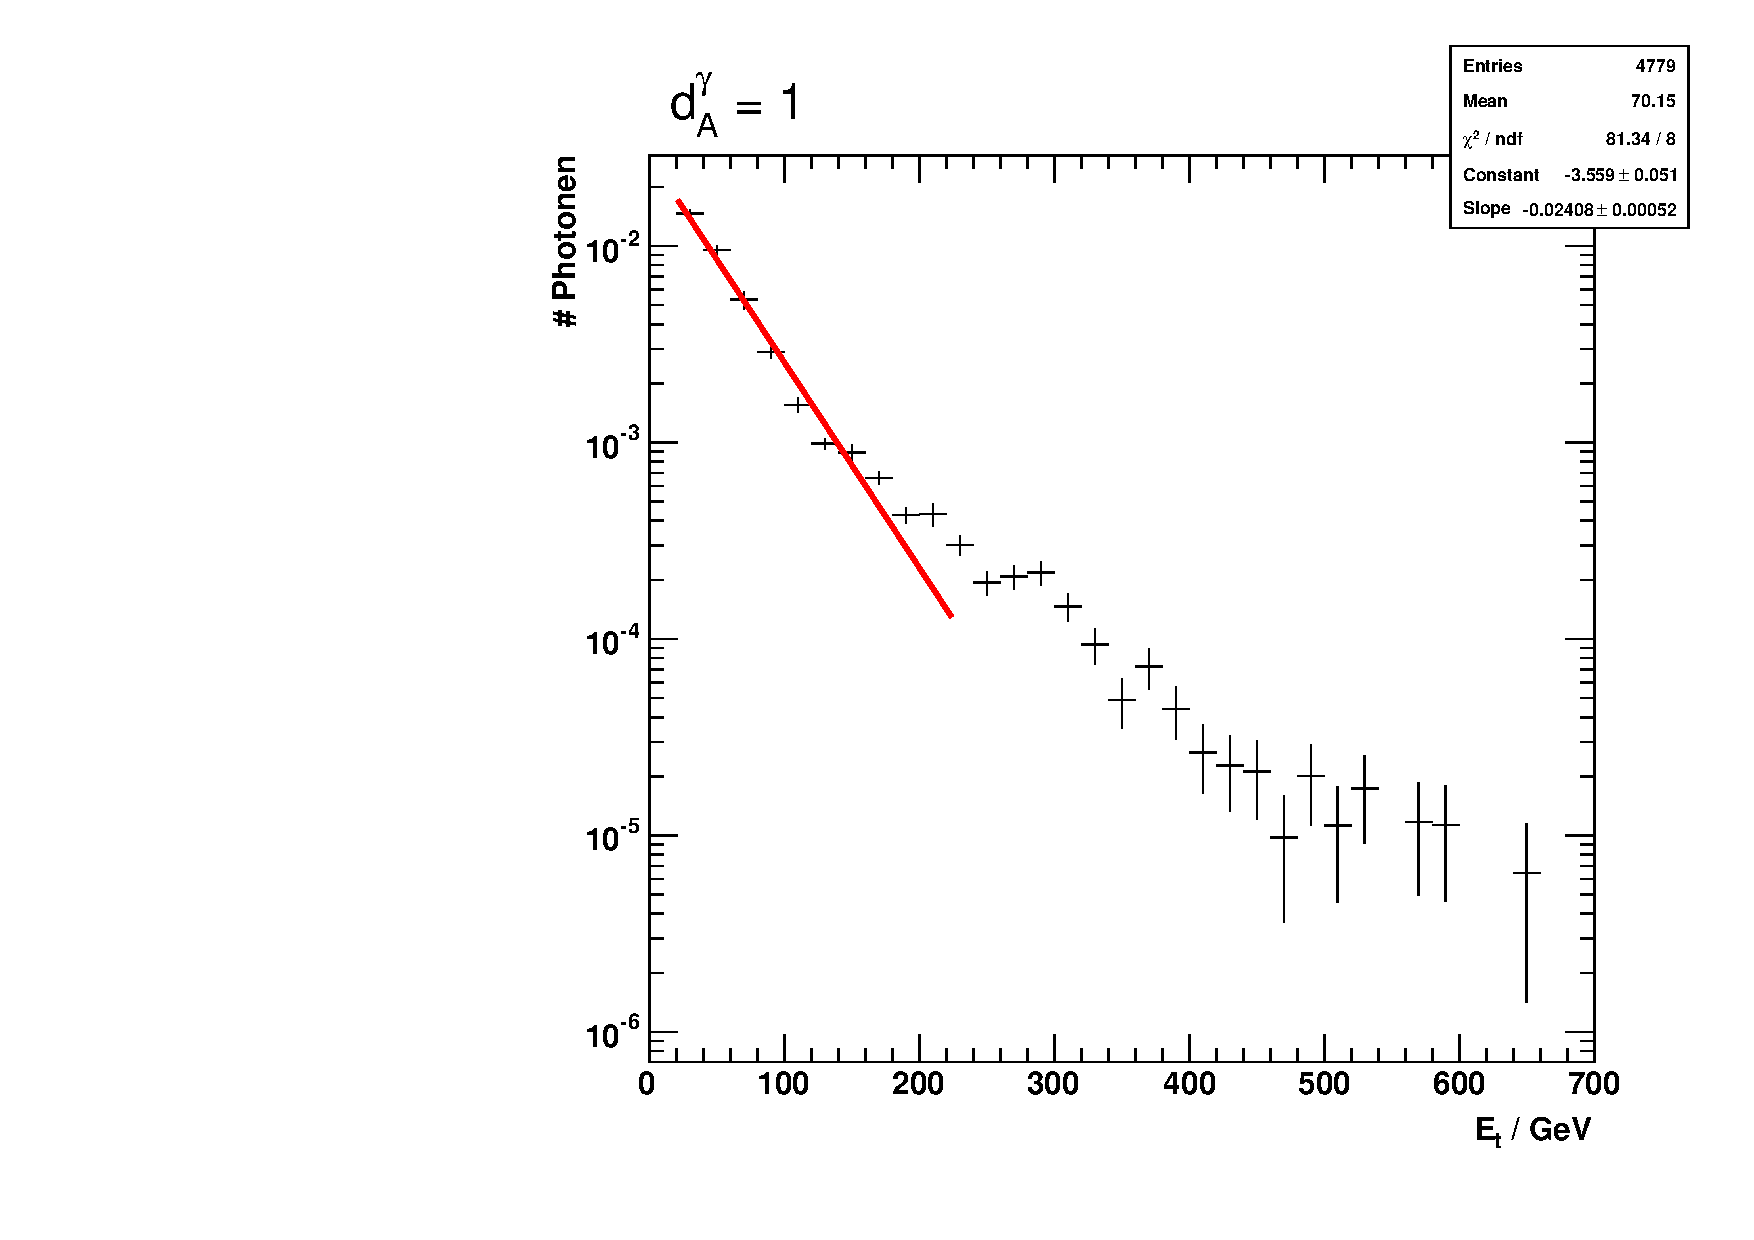
\includegraphics[width=\textwidth]{bilder/fit_1.pdf}%
\end{subfigure}
\caption{Exponentieller Fit an die $E_T$-Verteilungen von rekonstruierten und selektierten Monte-Carlo-Daten f�r verschiedene Werte von $d_A^{\gamma}$.}%
\label{fig:fit_galerie}%
\end{figure}


\begin{figure}%
\centering
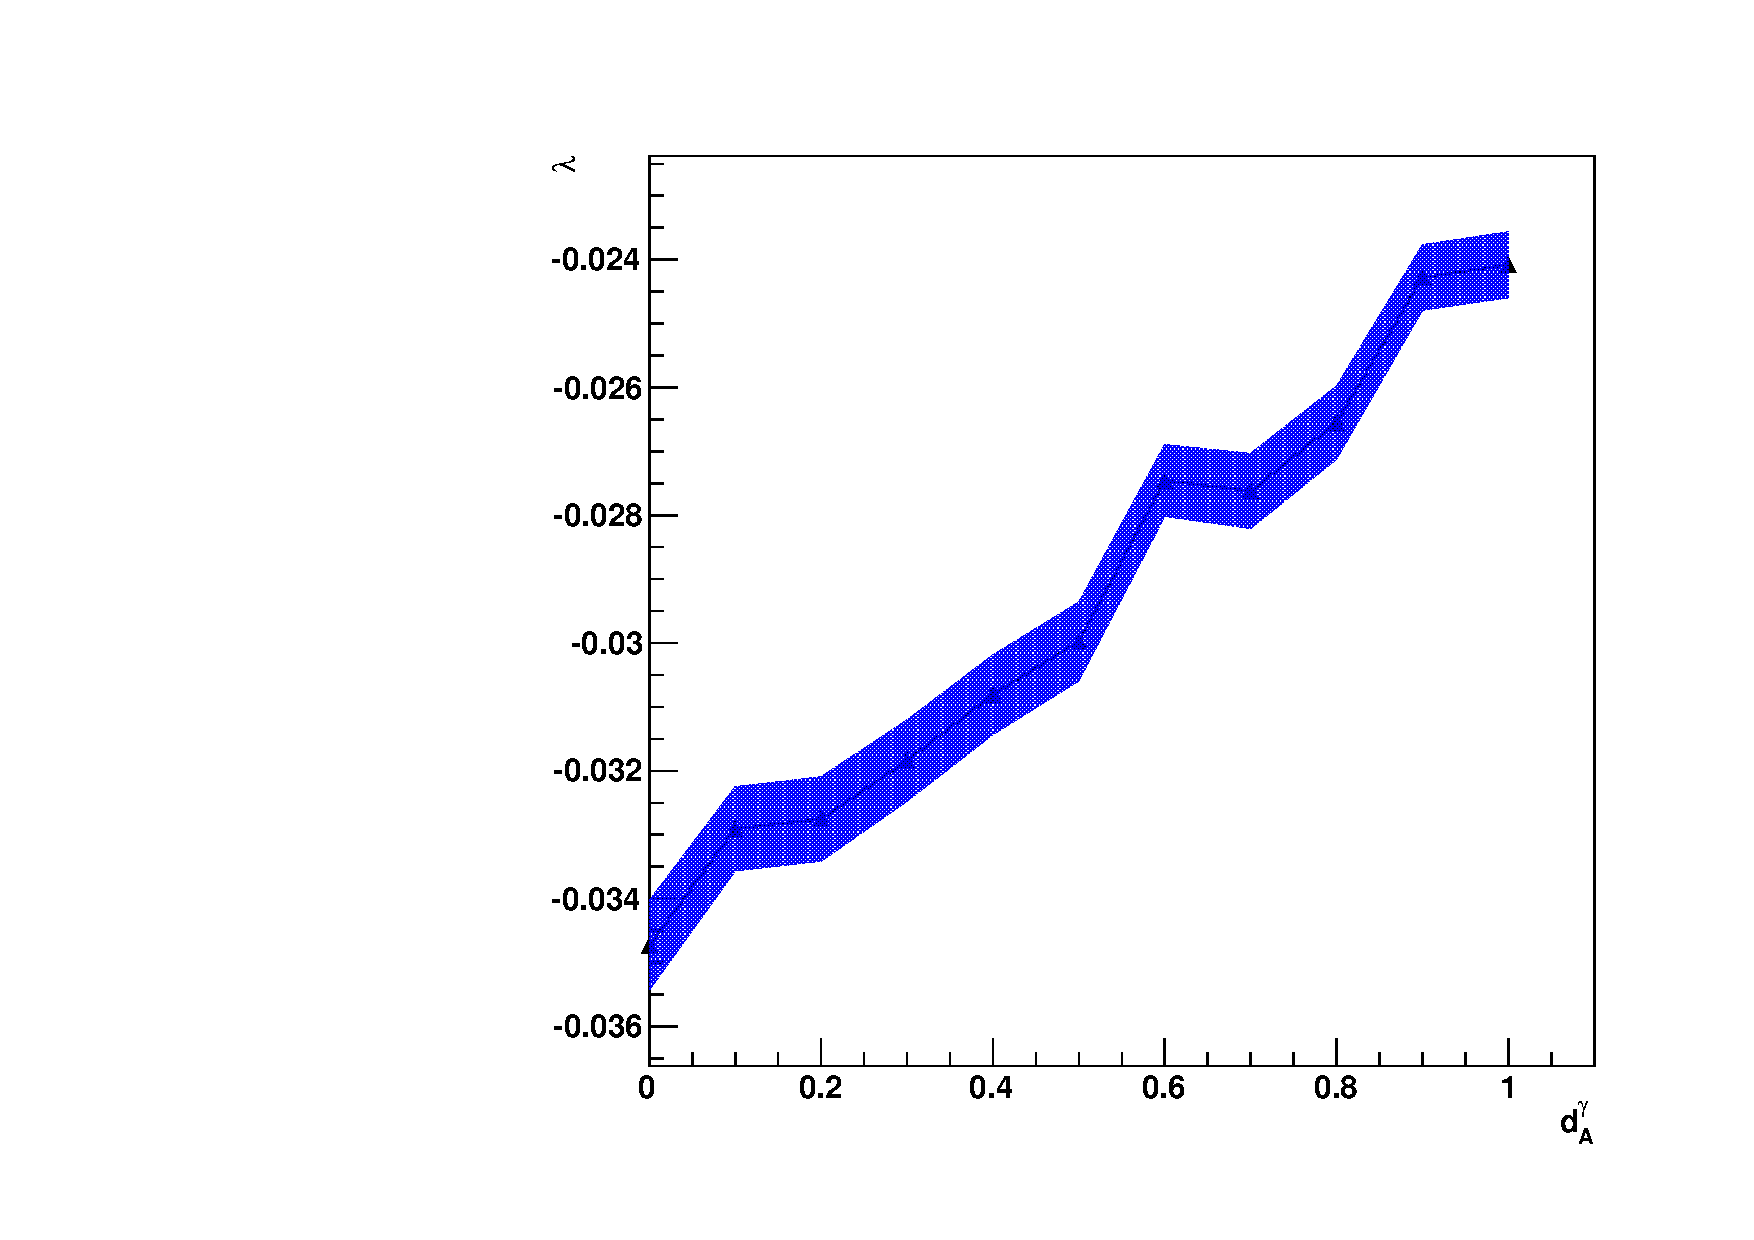
\includegraphics[width=0.5\columnwidth]{bilder/slope_reco_plot.pdf}%
\caption{}%
\label{fig:slope_reco_plot}%
\end{figure}

\section{Vergleich der Analysemethoden auf Rekonstruktionsniveau}

Auch bei der Analyse der rekonstruierten und selektierten Monte-Carlo-Ereignisse zeigt sich in allen vorgestellten Analysemethoden eine klare Abh�ngigkeit der jeweiligen Variablen von $d_A^{\gamma}$. Ebenso weisen alle Variablen eine Separationskraft auf, diese ist jedoch aufgrund der durch Rekonstruktion und Selektion verringerten Statistik kleiner als auf Generatorniveau. \\
Die gr��te Separationskraft auf Rekonstruktionsniveau zeigt die Analyse der Exponentialanpassung der $E_T$-Verteilung. Hier liegen zwischen den Extremwerten von $\overline{E_T}$ 15 Standardabweichungen. Die 2-Bin-Analyse weist einen Wertebereich von 10 Standardabweichungen auf und die Analyse des Schwerpunktes der Verteilung hat eine Spannweite von 9 Standardabweichungen. Somit hat die Analyse der Exponentialanpassung im Vergleich zum Generatorniveau nicht viel von ihrer Separationskraft eingeb��t. Die anderen beiden Analysemethoden separieren aufgrund der verringerten Statistik aber wie erwartet auf Rekonstruktionsniveau weitaus weniger stark zwischen den verschiedenen $d_A^{\gamma}$-Szenarien.

\section{Auswertung von 4,7 \texorpdfstring{fb$^{-1}$}{inv. fb} Daten}

Auf 4,7 fb$^{-1}$ Daten werden die gleichen Selektionen (Top-Paar- bzw. $t\overline{t} + \gamma$-Selektion) angewendet. Die Daten wurden im Jahr 2011 bei einer Schwerpunktsenergie von 7\,TeV genommen. Aus diesem Datensatz werden 134 Ereignisse selektiert, die alle geforderten Kriterien erf�llen. Das $E_T$-Spektrum dieser Ereignisse ist in Abbildung \ref{fig:et_data} gezeigt. \\

\begin{figure}%
\centering
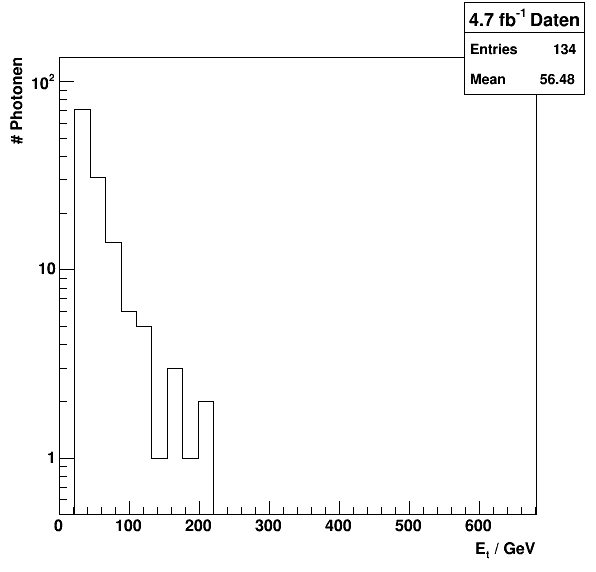
\includegraphics[width=0.4\columnwidth]{bilder/et_data}%
\caption{$E_T$-Verteilung von 4,7\,fb$^{-1}$ Daten aus 2011.}%
\label{fig:et_data}%
\end{figure}

Mit den oben beschriebenen Analysemethoden wird dieses Spektrum analog zu den Spektren aus Monte-Carlo-Simulationen untersucht. Dabei ergeben sich die folgenden Werte:

 \begin{itemize}
	 \item $(E_{Low}/E_{High})_{Data} = 5,09 \pm 1,19$
	 \item $\overline{E_T}_{Data} = 55,36 \pm 3,19\,GeV$
	 \item $\lambda_{Data} = -0,0333 \pm 0,0037$
 \end{itemize}

Um diese Werte mit den Verl�ufen aus den Monte-Carlo-Simulationen zu vergleichen, werden sie in die jeweiligen Plots eingef�gt, siehe Abbildung \ref{fig:ana_data_mc}.

\begin{figure}%
\centering
\begin{subfigure}[b]{0.4\textwidth}
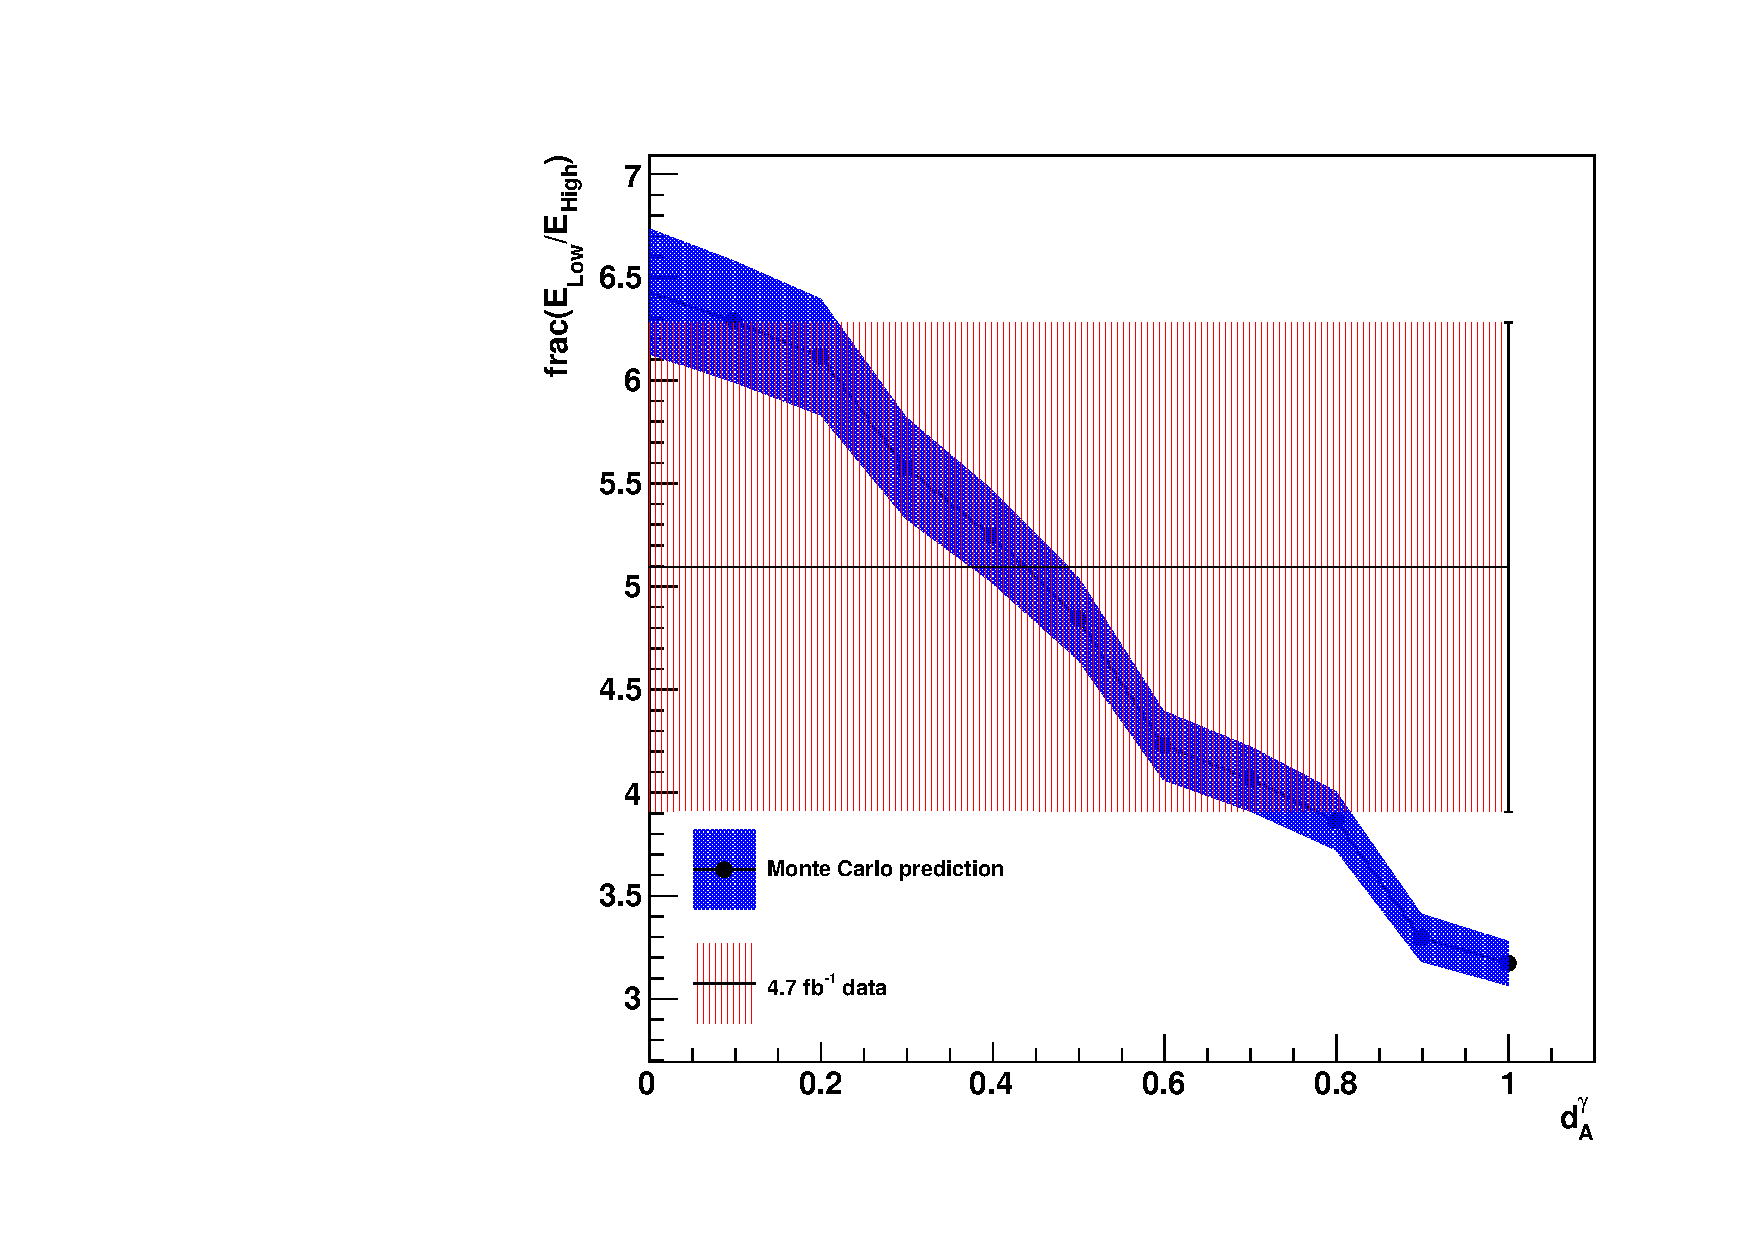
\includegraphics[width=\textwidth]{bilder/twobin_data_mc}%
\end{subfigure}
\hspace{0.1\textwidth}
\begin{subfigure}[b]{0.4\textwidth}
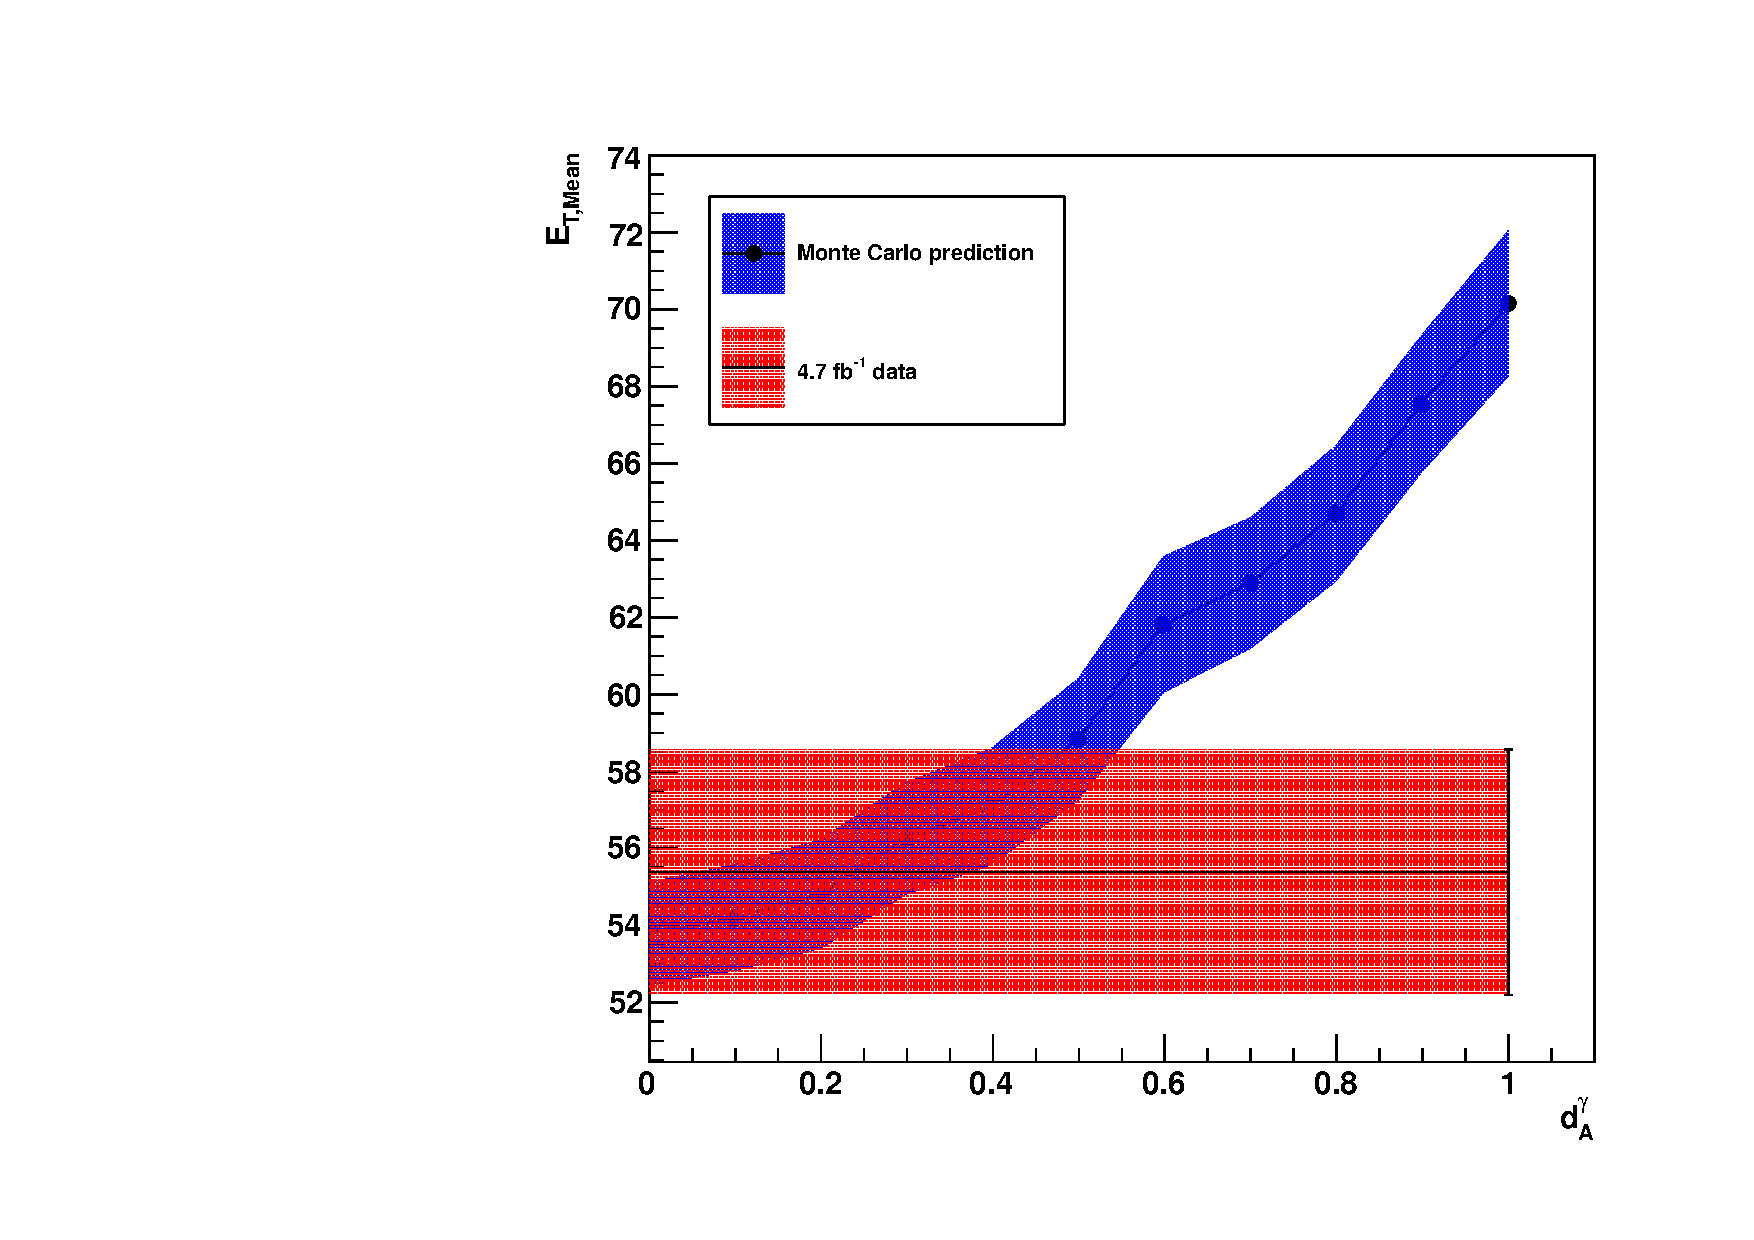
\includegraphics[width=\textwidth]{bilder/mean_data_mc}%
\end{subfigure}

\begin{subfigure}[b]{0.4\textwidth}
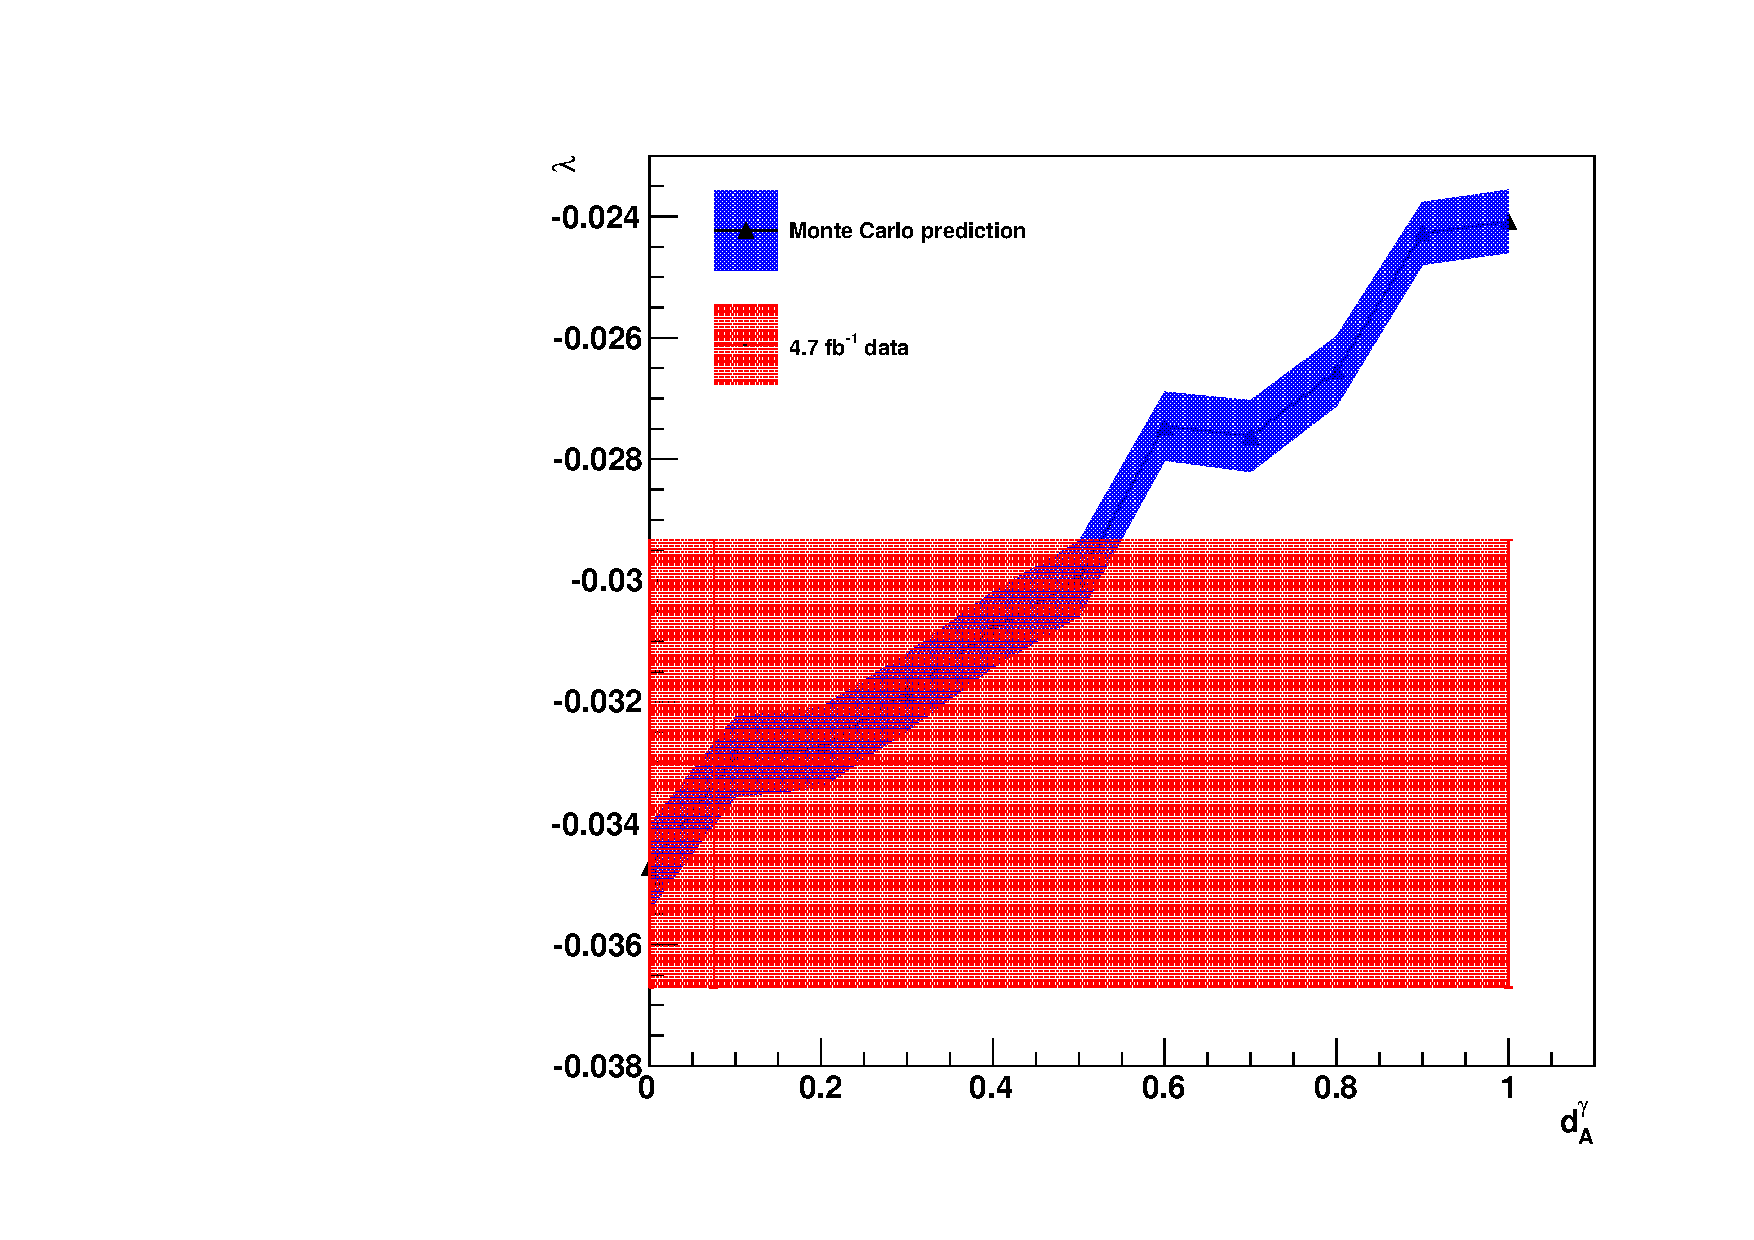
\includegraphics[width=\textwidth]{bilder/slope_data_mc}%
\end{subfigure}
\caption{Vergleich der Variablen f�r Monte-Carlo- und Daten-Ereignisse.}
\label{fig:ana_data_mc}
\end{figure}

In allen Analysemethoden ist ein gro�er statistischer Fehler auf die Werte f�r experimentell gesammelte Daten zu erkennen. Dies ist der kleinen Statistik von lediglich 134 Ereignissen geschuldet. Ebenso ist der Datenwert in allen Methoden mit dem Standardmodellwert von $d_A^{\gamma} = 0$ innerhalb einer Standardabweichung vereinbar, auf der anderen Seite liegen die Werte $d_A^{\gamma} > 0,6$ (Exponentialanpassung, Messung des Schwerpunktes) sowie $d_A^{\gamma} > 0,8$ au�erhalb des $1\sigma$-Bandes.

\section{Statistische und systematische Unsicherheiten der Analyse}

Die bis hierhin betrachteten Unsicherheiten sind alle ausschlie�lich statistischer Natur. Es treten jedoch auch systematische UNsicherheiten auf. Im Folgenden werden die statistischen und systematischen Unsicherheiten n�her betrachtet.

\subsection{Statistische Unsicherheiten}

Die statistischen Unsicherheiten auf die Variablen $E_{Low}/E_{High}$, $\overline{E_T}$ und $\lambda$ werden folgendermassen bestimmt:

\begin{description}
  \item [$E_{Low}/E_{High}$] Die Unsicherheit auf die Bininhalte $E_{Low}$ und $E_{High}$ wird mit $\sqrt{E_{Low}}$ beziehungsweise $\sqrt{E_{High}}$ angenommen und der Unsicherheit auf das Verh�ltnis mittels Gauss'scher Fehlerfortpflanzung berechnet.
	\item [$\overline{E_T}$] Die Unsicherheit auf den Schwerpunkt der $E_T$-Verteilung wird mittels Formel \ref{eq:meanerror} berechnet.
	\item [$\lambda$] Die Unsicherheit auf den Parameter der Exponentialanpassung wird mittels der in Kapitel \ref{sec:ensemble} beschriebenen Ensemblestudie durch 1000faches Neuw�rfeln der $E_T$-Verteilung bestimmt.
\end{description}

\subsection{Systematische Unsicherheiten}
\label{sec:systematiken}

Die Analyse wird von vielen systematischen Effekten limitiert. Exemplarisch wird hier die Abh�ngigkeit von der Wahl des Monte-Carlo-Generators und der Einfluss der Normierung der Signal- bzw. Untergrund-Sample diskutiert. Die Zahlenwerte gelten jeweils f�r das $d_A^{\gamma} = 0$-Szenario.

\begin{description}
  \item [Generator] Verschiedene Monte-Carlo-Generatoren benutzen unterschiedliche Algorithmen zur Simulation der Hadronisierung und Schauerbildung und erzeugen somit auch voneinander abweichende Energiespektren. Ein zweites $t\overline{t}$-Sample wurde mit einem anderen Matrixelementgenerator (MC@NLO) und einem anderen Hadronisierungs- und Schauermodell (HERWIG) generiert. Dieses wurde mit einem Sample verglichen, welches mittels MADGRAPH und PYTHIA, wie in dieser Analyse verwendet, mit denselben Randbedingungen erstellt wurde. Die volle Photon-$E_T$-Analyse wurde mit beiden Samplen durchgef�hrt und die relative Abweichung der untersuchten Variablen als systematische Unsicherheit definiert:
	
	\begin{equation}
	\Delta X_{rel} = \frac{X_{MC@NLO}-X_{MADGRAPH}}{X_{MADGRAPH}} \ .
	\end{equation}

Hier bezeichnet X die jeweils untersuchte Variable.
  \item [Normalisierung des Signals] Die Unsicherheit aufgrund der Signalnormalisierung wird bestimmt, indem die Ereigniszahl des Signal-Samples um $\pm 25\%$ variiert wird. Dies bildet eine �nderung der Faktorisierungs- beziehungsweise Renormalisierungsskala ab.
	\item [Normalisierung der Untergr�nde] Die in Kapitel \ref{sec:top_untergrund} beschriebenen Unsicherheiten auf den Wirkungsquerschnitt der Untergrundsignale werden gaussisch addiert und die Ereigniszahl der Untergrundprozesse mit dieser Gesamtunsicherheit variiert.
\end{description}

Es ergeben sich damit f�r die untersuchten Variablen im $d_A^{\gamma} = 0$-Szenario die folgenden Werte:

\begin{itemize}
	\item $E_{Low}/E_{High} = 6,421 \pm 0,304 (\text{stat.}) \pm 0,841 (\text{syst.})$
	\item $\overline{E_T} = 53,745 \pm 1,331 (\text{stat.}) \pm 1,381 (\text{syst.})$\,GeV
	\item $\lambda = -0,03473 \pm 0,00070 (\text{stat.}) \pm 0,00208 (\text{syst.})$
\end{itemize}